\documentclass{beamer}

\usepackage{amsmath}
\usepackage{amssymb}
\usepackage{amsthm}
\usepackage{mathtools}
\usepackage[UKenglish]{babel}
\usepackage{enumerate}
\usepackage{graphicx}
\usepackage{braket}
\usepackage{esint}
\usepackage{float}
\usepackage{tabularx}
\usepackage{array}
\usepackage{subcaption}
\usepackage{hyperref}
\hypersetup{colorlinks=false, bookmarks=true}

\usetheme{Madrid}
\usecolortheme{seahorse}
\usefonttheme{professionalfonts}
\useinnertheme{circles}

\AtBeginSection[]
{
  \begin{frame}
    \frametitle{Table of Contents}
    \tableofcontents[currentsection]
  \end{frame}
}

\setbeamertemplate{caption}[numbered]

\title[QCNN State Preparation]{A QCNN for Quantum State Preparation}
\subtitle{Carnegie Vacation Scholarship}
\author[David Amorim]{David Amorim}
\institute[]{}
\date[29/07/2024]{Week 4 \\(22/07/2024 - 26/07/2024)}

\begin{document}

\frame{\titlepage}

\section{Preliminaries}
\begin{frame}
\frametitle{Aims for the Week}
The following aims were set at the last meeting (22/07/2024):

\begin{alertblock}{Change Input Layer Structure}
Improve the connectivity of input layers. Each input qubit should ideally control each target qubit at some point in the network. 
\end{alertblock}

\begin{alertblock}{Fix Parameters}
Add the option to keep parameters fixed for each type of network layer. 
\end{alertblock}

\begin{alertblock}{Improve Loss Function}
Develop a distance measure taking into account digital encoding. Either incorporate this into weights for an existing loss function or define a new loss function on this basis. 
\end{alertblock}
\end{frame}

\begin{frame}
\frametitle{Additional Aim: Understanding Phase Extraction}
\begin{itemize}
\item Phase encoding is based on two operators, \alert{$\hat{Q}_\Psi$ and $\hat{R}$}, defined via 
\begin{align}
\hat{Q}_\Psi \ket{j}\ket{0} &= \ket{j}\ket{\Psi(j)} \\
\hat{R} \ket{l} &= e^{i l} \ket{l}
\end{align}
\item Encoding proceeds in \alert{three steps}:
\begin{equation}
\ket{j}\ket{0}\xmapsto{\alert{\hat{Q}_\Psi}} \ket{j}\ket{\Psi(j)} \xmapsto{\alert{\hat{I} \otimes \hat{R}}} \ket{j} e^{i \Psi(j)} \ket{\Psi(j)} \xmapsto{\alert{\hat{Q}_\Psi^\dagger}} e^{i \Psi (j)} \ket{j} \ket{0}, 
\end{equation}
\item The phase $e^{i \Psi (j)}$ of the final state is extracted \alert{assuming the ancilla register is clear} (i.e. in the state $\ket{0}$)
\item However, when $\hat{Q}_\Psi$ does not produce an eigenstate of $\hat{I} \otimes \hat{R}$, applying $\hat{Q}^\dagger$ does not generally clear the ancilla
\item  A flawed implementation of $\hat{Q}_\Psi$ \alert{non-trivially affects the extracted phase function} 
\end{itemize}
\end{frame}

\begin{frame}
\frametitle{Additional Aim: Understanding Phase Extraction}
\begin{itemize}
\item To investigate this relationship between $\hat{Q}_\Psi$ and the extracted phase (`\alert{phase extraction problem}'), make the following definitions:
\begin{itemize}
\item $\mathsf{M}_j$:  mismatch between $\ket{j} \ket{\Psi(j)}$ and $\hat{Q}_\Psi \ket{j}\ket{0}$
\item $\ket{\psi}_\text{final}$: state vector post phase extraction 
\item $\tilde{\Psi}$: extracted phase function  (in contrast to the target function, $\Psi$)
\end{itemize}
\item Based on the above, define \alert{five metrics} that quantify the quality of $\hat{Q}_\Psi$ as well as of phase extraction:
\end{itemize}

\begin{table}
\begin{tabular}{c | c | c | c}
& \textbf{Definition} & \textbf{Description} & \textbf{Ideal Value} \\ \hline 
$\boldsymbol{\mu}$ & $\text{Mean}(\mathsf{M}_j)$ & mean mismatch & 0  \\
$\boldsymbol{\sigma}$ &  $\text{STDEV}(\mathsf{M}_j)$ & mismatch STDEV & 0  \\
$\boldsymbol{\epsilon}$ & $1 - |\braket{\psi | \psi}_\text{final}|^2$ & normalisation error & 0 \\ 
$\boldsymbol{\chi}$ &  $\text{Mean}(|\tilde{\Psi}(j) - \Psi(j)|)$ & phase function error & 0 \\
$\boldsymbol{\Omega}$ & $\left( \mu + \sigma + \epsilon + \chi \right)^{-1}$ & super-metric & $\infty$
\end{tabular}
\caption{Metrics introduced to quantify QCNN performance}
\end{table}

\end{frame}

\begin{frame}
\frametitle{Glossary}
\begin{table}
\begin{center}
\begin{tabularx}{\textwidth}{ c|>{\centering}X}
  \textbf{Acronym} & \textbf{Meaning} \tabularnewline
  \hline 
  CL  & convolutional layer   \tabularnewline
  AA-CL  & all-to-all convolutional layer \tabularnewline
  NN-CL  & neighbour-to-neighbour convolutional layer \tabularnewline
  IL & input layer \tabularnewline 
  SAM & sign-adjusted mismatch
\end{tabularx}
\caption{Acronyms used in the following.}
\end{center}
\end{table}
\begin{table}
\begin{center}
\begin{tabularx}{\textwidth}{>{$}c<{$}|>{\centering}X}
  \textbf{Variable} & \textbf{Meaning} \tabularnewline
  \hline 
  n  & input register size   \tabularnewline
  m  &  target register size \tabularnewline
  L  & number of network layers \tabularnewline
  \Psi_\text{H23} & phase function from Hayes 2023
\end{tabularx}
\caption{Variables used in the following.}
\end{center}
\end{table}
\end{frame}

\section{Changing Input Layer Structure}

\begin{frame}
\frametitle{Changing Input Layer Structure}
\begin{itemize}
\item Previously, the $j$th input qubit controlled an operation on the $j$th target qubit (with wrap-around for $n >m$) 
\item An optional \alert{shift parameter}, $s$, has now been added so that the $j$th input qubit controls an operation on the $j+s$th target qubit 
\item This shift parameter is incremented for each successive IL 
\item The QCNN is padded with additional ILs to ensure that the number of ILs is $\geq m$ 
\item Thus, \alert{each input qubit now controls an operation on each target qubit} at some point in the QCNN 
\item Note that ILs still alternate between control states 0 and 1
\end{itemize}.
\end{frame}

\begin{frame}
\frametitle{Changing Input Layer Structure}
\begin{columns}
\begin{column}{0.5\textwidth}
\begin{table}
\begin{tabular}{c || c| c }
& shifts & no shifts \\ \hline \hline 
$\mu$ & 3.4e-2 & \alert{\textbf{3.2e-2}}  \\
$\sigma$ & \textbf{1.4e-1} & 1.5e-1  \\
$\epsilon$  & \textbf{2.0e-2} & 7.5e-2 \\
$\chi$ & \textbf{3.2e-2} & 1.3e-0    \\ \hline 
$\Omega$ &  \textbf{ 4.46} & 0.63
\end{tabular}
\caption{Comparing metrics for $\Psi(f) \sim f$ ($L=6$, $m=3$, 600 epochs, SAM)}
\end{table}
\end{column}
\begin{column}{0.5\textwidth}
\begin{figure}
\centering 
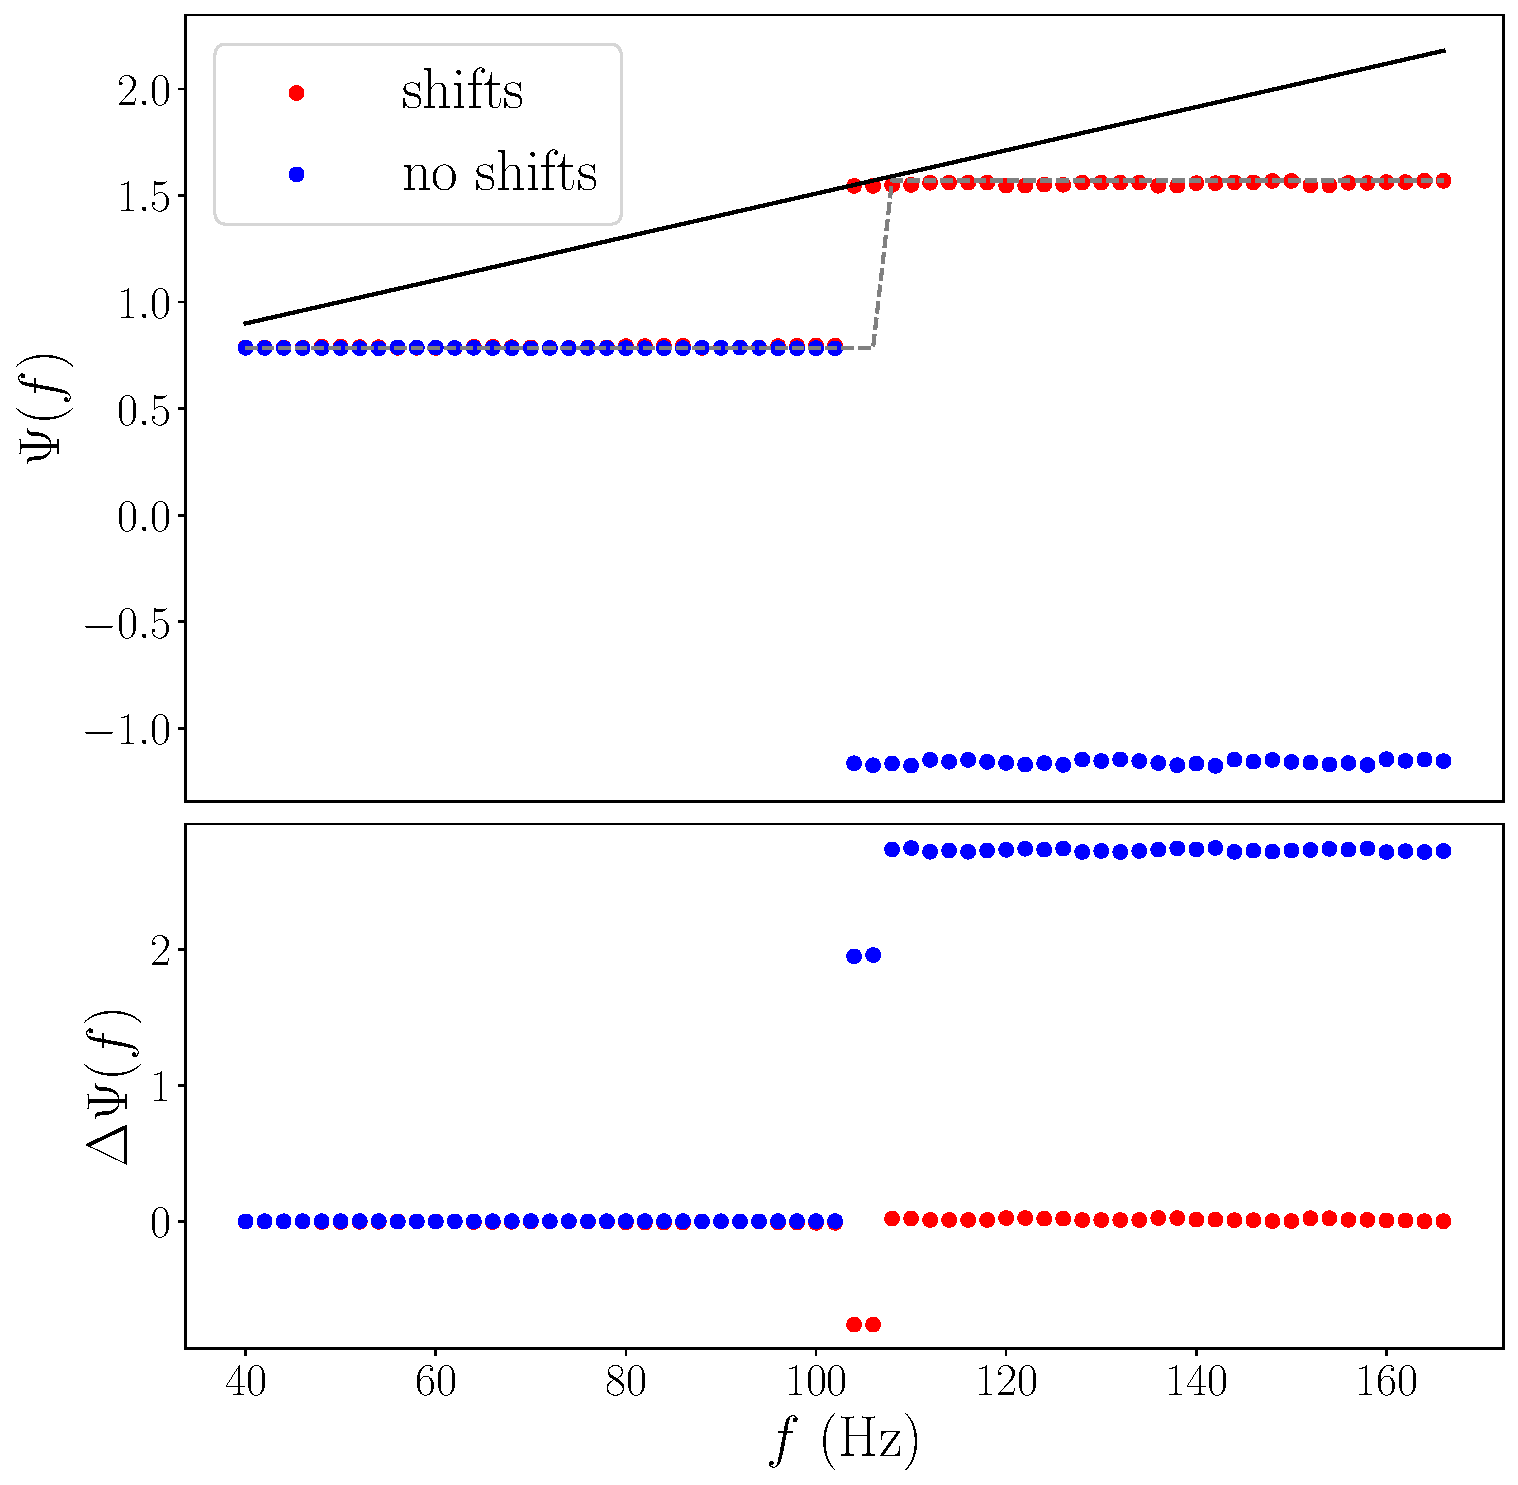
\includegraphics[width=\textwidth]{im/phase_shift_comp_linear_m3}
\caption{Effects of shifted ILs for $\Psi(f) \sim f$ ($L=6$, $m=3$, 600 epochs, SAM)}
\end{figure}
\end{column}
\end{columns}
\end{frame}

\begin{frame}
\frametitle{Changing Input Layer Structure}
\begin{columns}
\begin{column}{0.5\textwidth}
\begin{table}
\begin{tabular}{c || c| c }
& shifts & no shifts \\ \hline \hline 
$\mu$ & \textbf{1.9e-1} & 2.4e-1   \\
$\sigma$ & \textbf{1.2e-1} & 1.5e-1  \\
$\epsilon$  & \textbf{2.2e-1} & 4.7e-1 \\
$\chi$ &\textbf{ 1.9e-1} & 4.3e-1 \\ \hline 
$\Omega$ & \textbf{1.39} &  0.78 
\end{tabular}
\caption{Comparing metrics for $\Psi(f) \sim f^2$ ($L=6$, $m=3$, 600 epochs, SAM)}
\end{table}
\end{column}
\begin{column}{0.5\textwidth}
\begin{figure}
\centering 
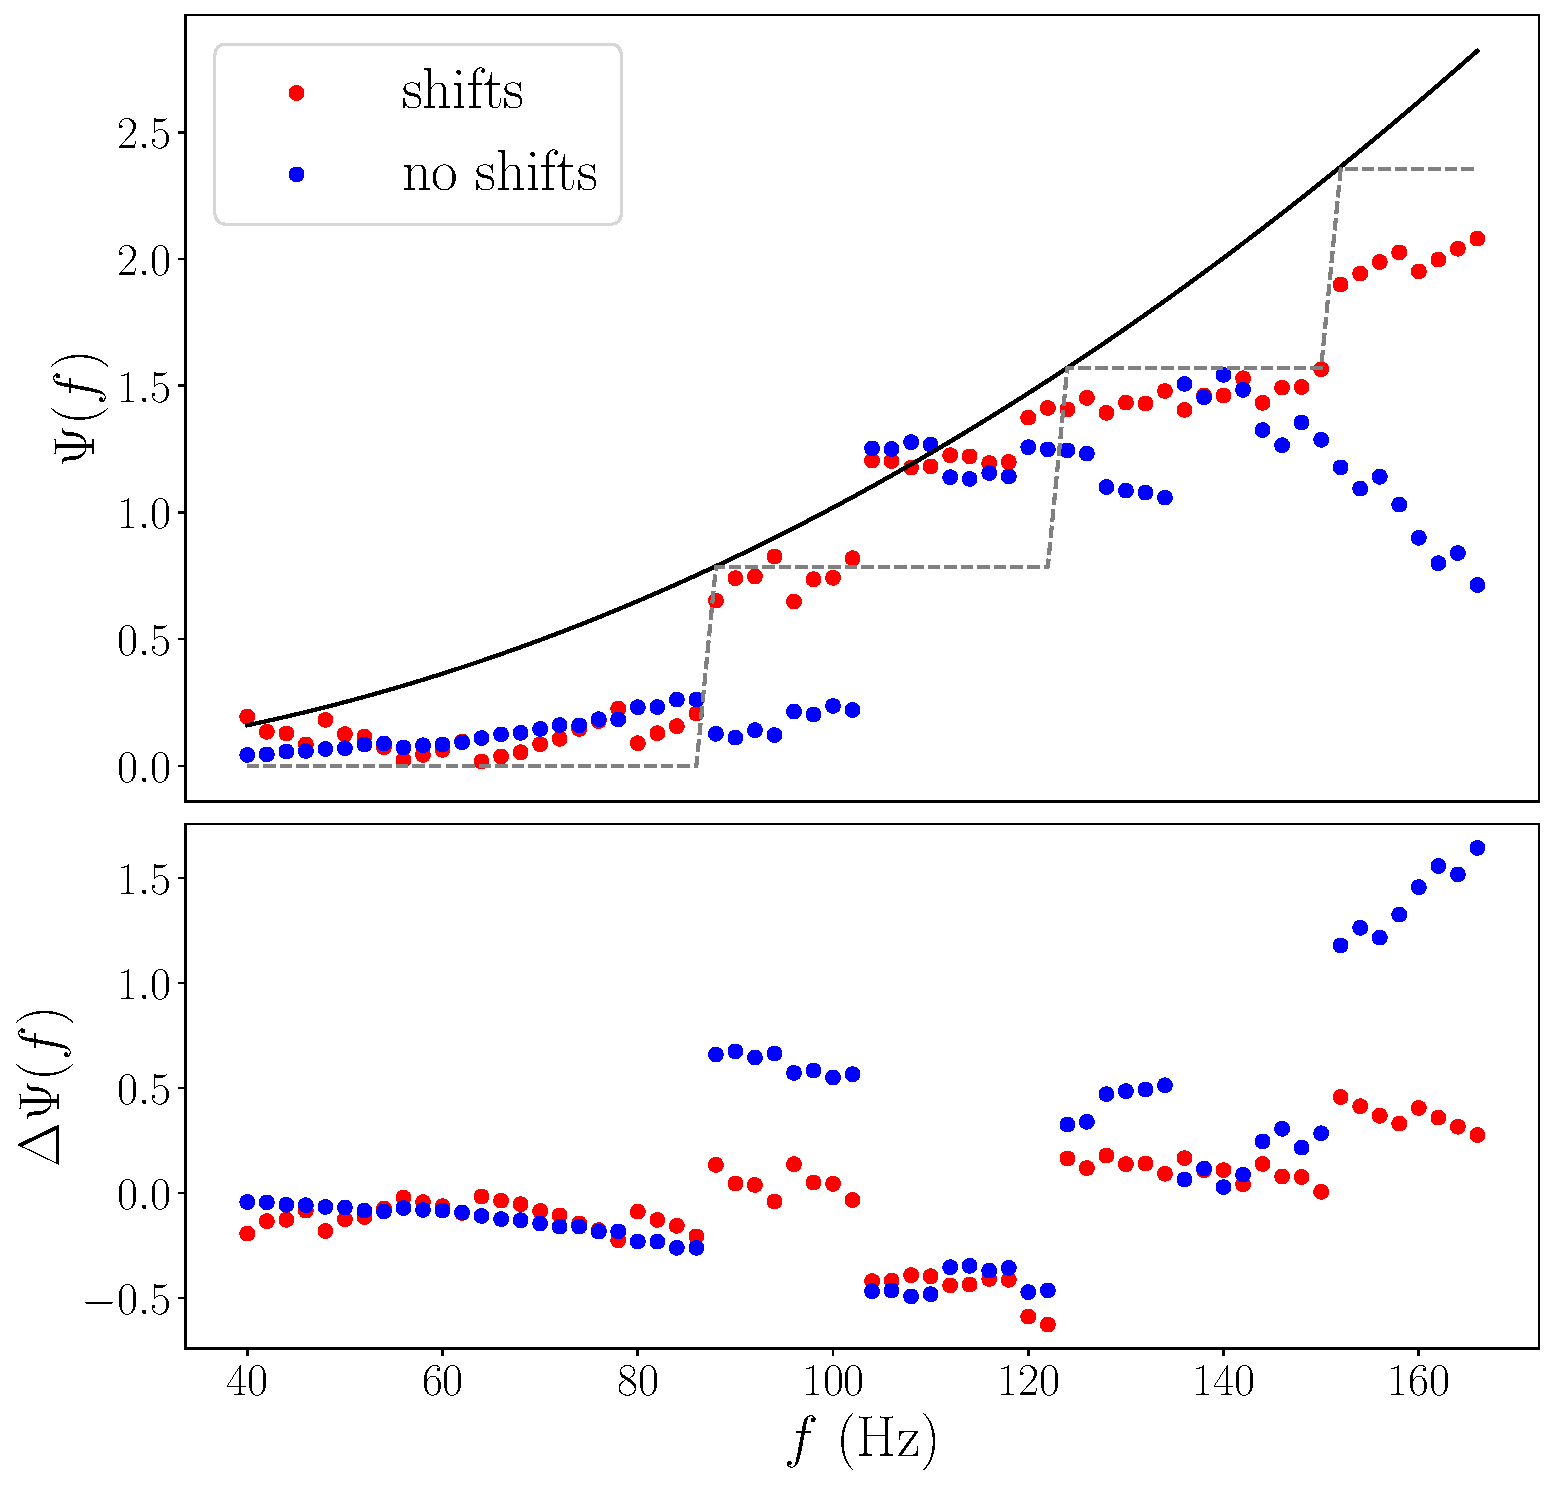
\includegraphics[width=\textwidth]{im/phase_shift_comp_quadratic_m3}
\caption{Effects of shifted ILs for $\Psi(f) \sim f^2$ ($L=6$, $m=3$ ,600 epochs, SAM)}
\end{figure}
\end{column}
\end{columns}
\end{frame}

\begin{frame}
\frametitle{Changing Input Layer Structure}
\begin{columns}
\begin{column}{0.5\textwidth}
\begin{itemize}
\item The data for `no shifts' was obtained by setting  $s=0$ for all ILs instead of incrementing $s$
\item This corresponds to last week's circuit structure of each input qubit controlling precisely one target qubit
\item Clearly, \alert{increased IL connectivity leads to improved performance}
\end{itemize}
\end{column}
\begin{column}{0.5\textwidth}
\begin{figure}
\centering 
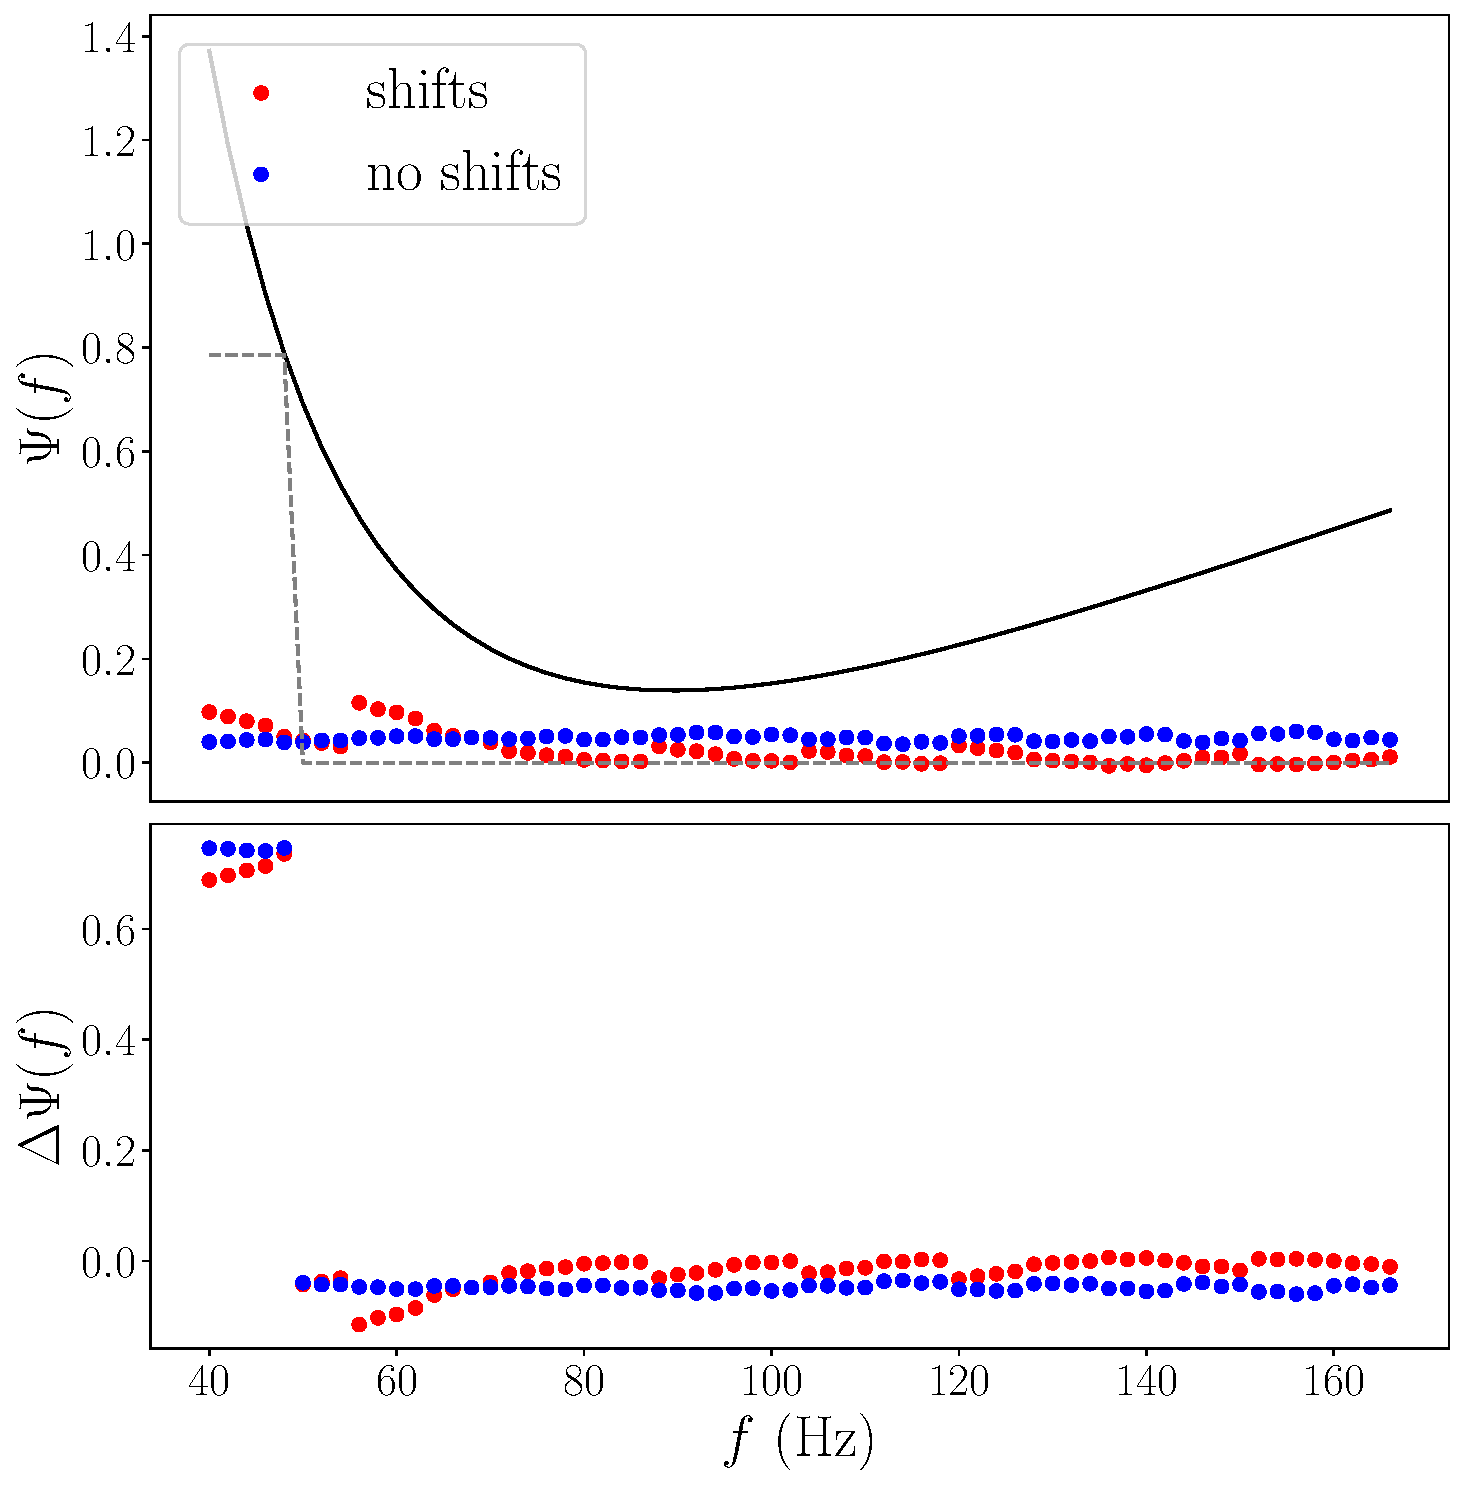
\includegraphics[width=\textwidth]{im/phase_shift_comp_psi_m3}
\caption{Effects of shifted ILs for $\Psi_\text{H23}$ ($L=6$, $m=3$, 600 epochs, SAM)}
\end{figure}
\end{column}
\end{columns}
\end{frame}


\section{Fixing Parameters}

\begin{frame}
\frametitle{Fixing Parameters}
\begin{itemize}
\item Implemented the option to \alert{fix parameters for each layer type}
\item This means that each instance of a layer type (IL, AA-CL, NN-CL) uses the same set of parameters 
\item This \alert{reduces the number of trainable parameters}, particularly at large $L$
\item Surprisingly, reducing the parameter space \alert{produces no noticeable speed-up} (so-called qiskit primitives, i.e. the sampler, take up roughly 95\% of the computational time)
\end{itemize}
\end{frame}

\begin{frame}
\frametitle{Fixing Parameters}
\begin{columns}
\begin{column}{0.52\textwidth}
\begin{table}
\begin{tabular}{c || c| c | c| c }
&none & CL & IL & both \\ \hline \hline 
$\mu$ & \textbf{1.3e-1} & 1.5e-1 & 4.5e-1 & 4.4e-1   \\
$\sigma$ & 2.2e-1 & \textbf{2.1e-1} & 2.6e-1 & 1.6e-1  \\
$\epsilon$  & \textbf{4.4e-2} & 1.5e-1 & 4.9e-1 & 5.8e-1 \\
$\chi$ & \textbf{6.8e-2} & 8.0e-2 & 2.4e-1 & 2.3e-1 \\ \hline 
$\Omega$ & \textbf{2.14} & 1.68 & 0.70 & 0.71 
\end{tabular}
\caption{Comparing metrics for $\Psi(f) \sim f$ ($L=6$, $m=4$, 600 epochs, SAM)}
\end{table}
\end{column}
\begin{column}{0.48\textwidth}
\begin{figure}
\centering 
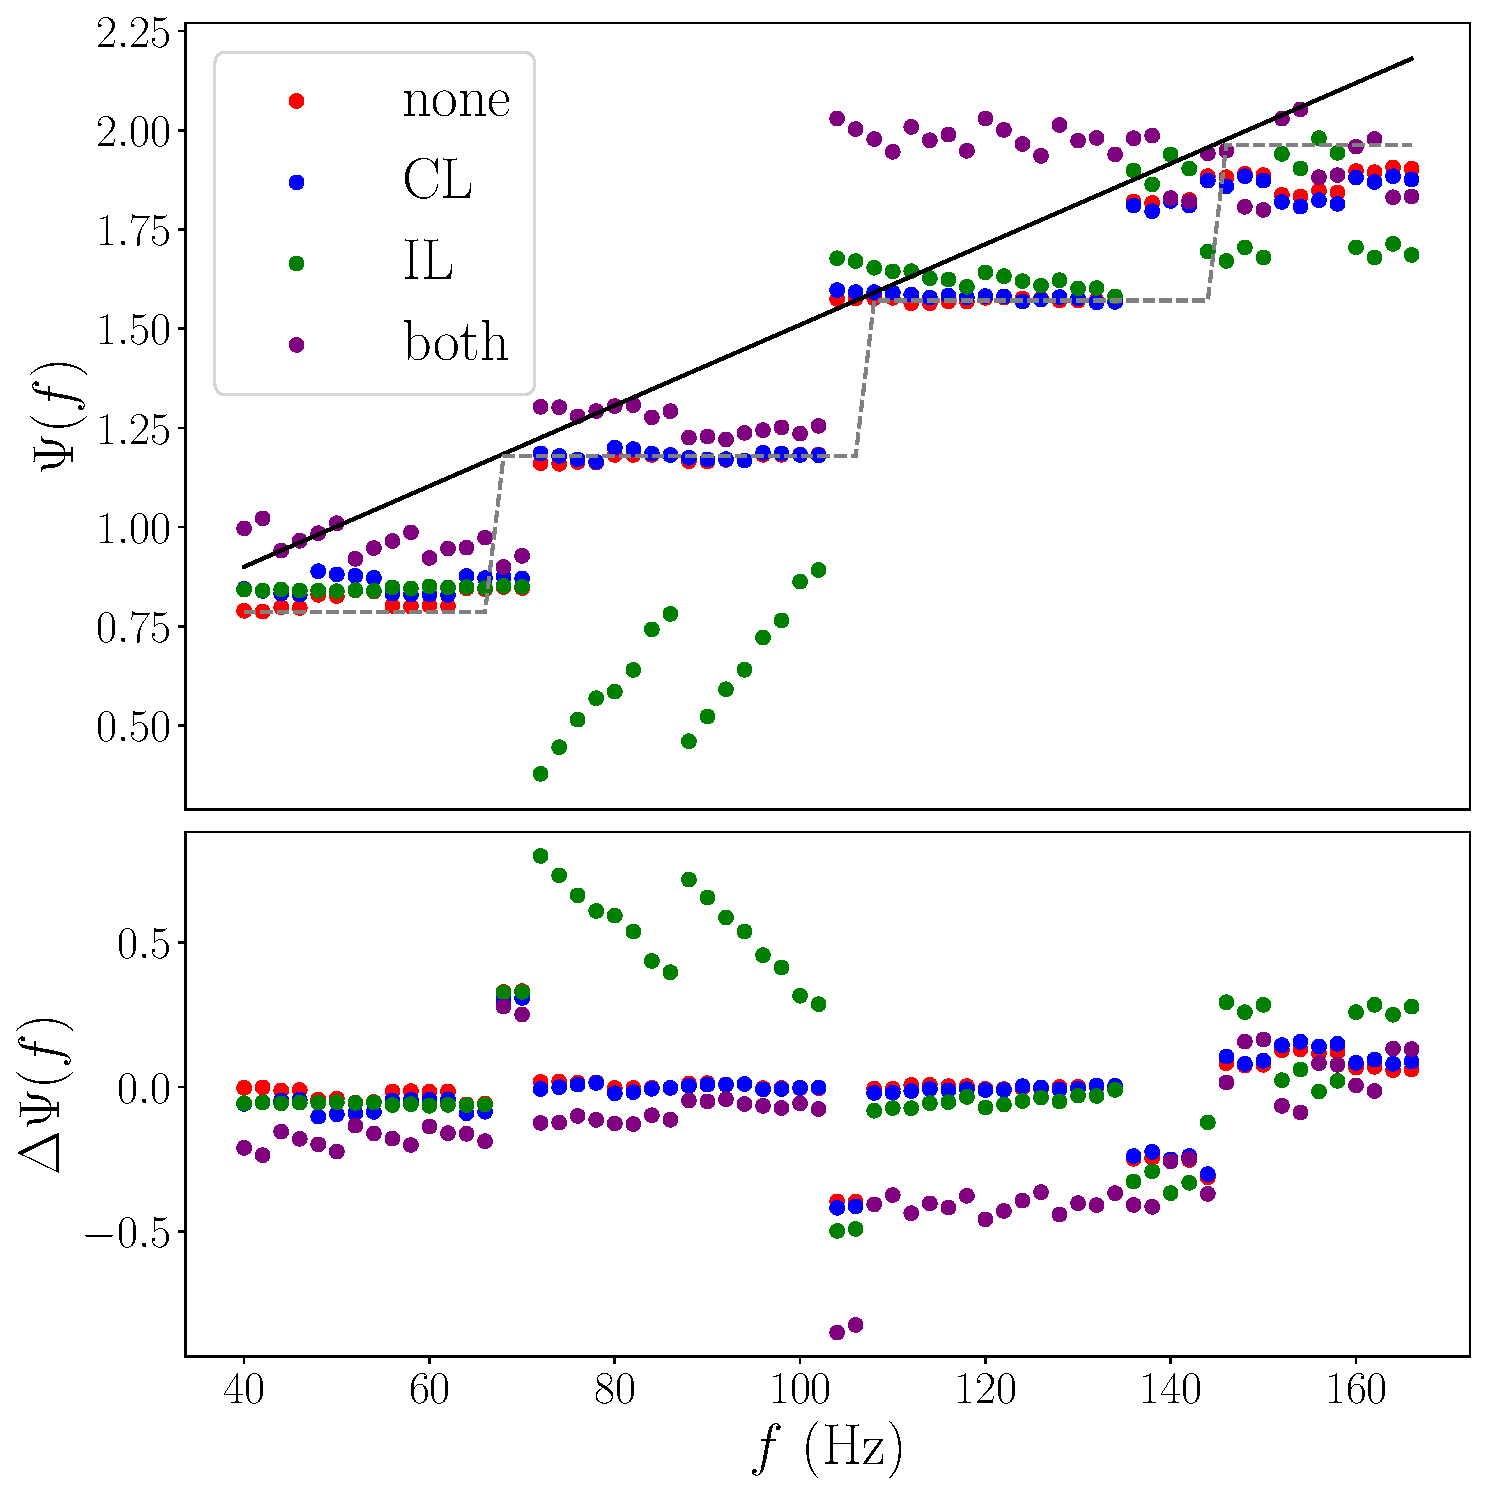
\includegraphics[width=\textwidth]{im/phase_RP_comp_linear_m4}
\caption{Effects of fixing parameters ILs for $\Psi(f) \sim f$ ($L=6$, $m=4$, 600 epochs, SAM)}
\end{figure}
\end{column}
\end{columns}
\end{frame}

\begin{frame}
\frametitle{Fixing Parameters}
\begin{columns}
\begin{column}{0.52\textwidth}
\begin{table}
\begin{tabular}{c || c| c | c| c }
&none & CL & IL & both \\ \hline \hline 
$\mu$ & \textbf{2.3e-1} & 3.5e-1 & 5.8e-1 & 5.3e-1   \\
$\sigma$ & \textbf{1.3e-1} & 1.6e-1 & 2.5e-1 & 2.0e-1  \\
$\epsilon$  &\textbf{ 2.7e-1} & 4.4e-1 & 4.3e-1 & 3.3e-1 \\
$\chi$ & \textbf{1.7e-1} & 1.8e-1 & 1.9e-0 & 3.6e-1 \\ \hline 
$\Omega$ & \textbf{1.26} & 0.88 & 0.32 & 0.71
\end{tabular}
\caption{Comparing metrics for $\Psi(f) \sim f^2$ ($L=6$, $m=4$, 600 epochs, SAM)}
\end{table}
\end{column}
\begin{column}{0.48\textwidth}
\begin{figure}
\centering 
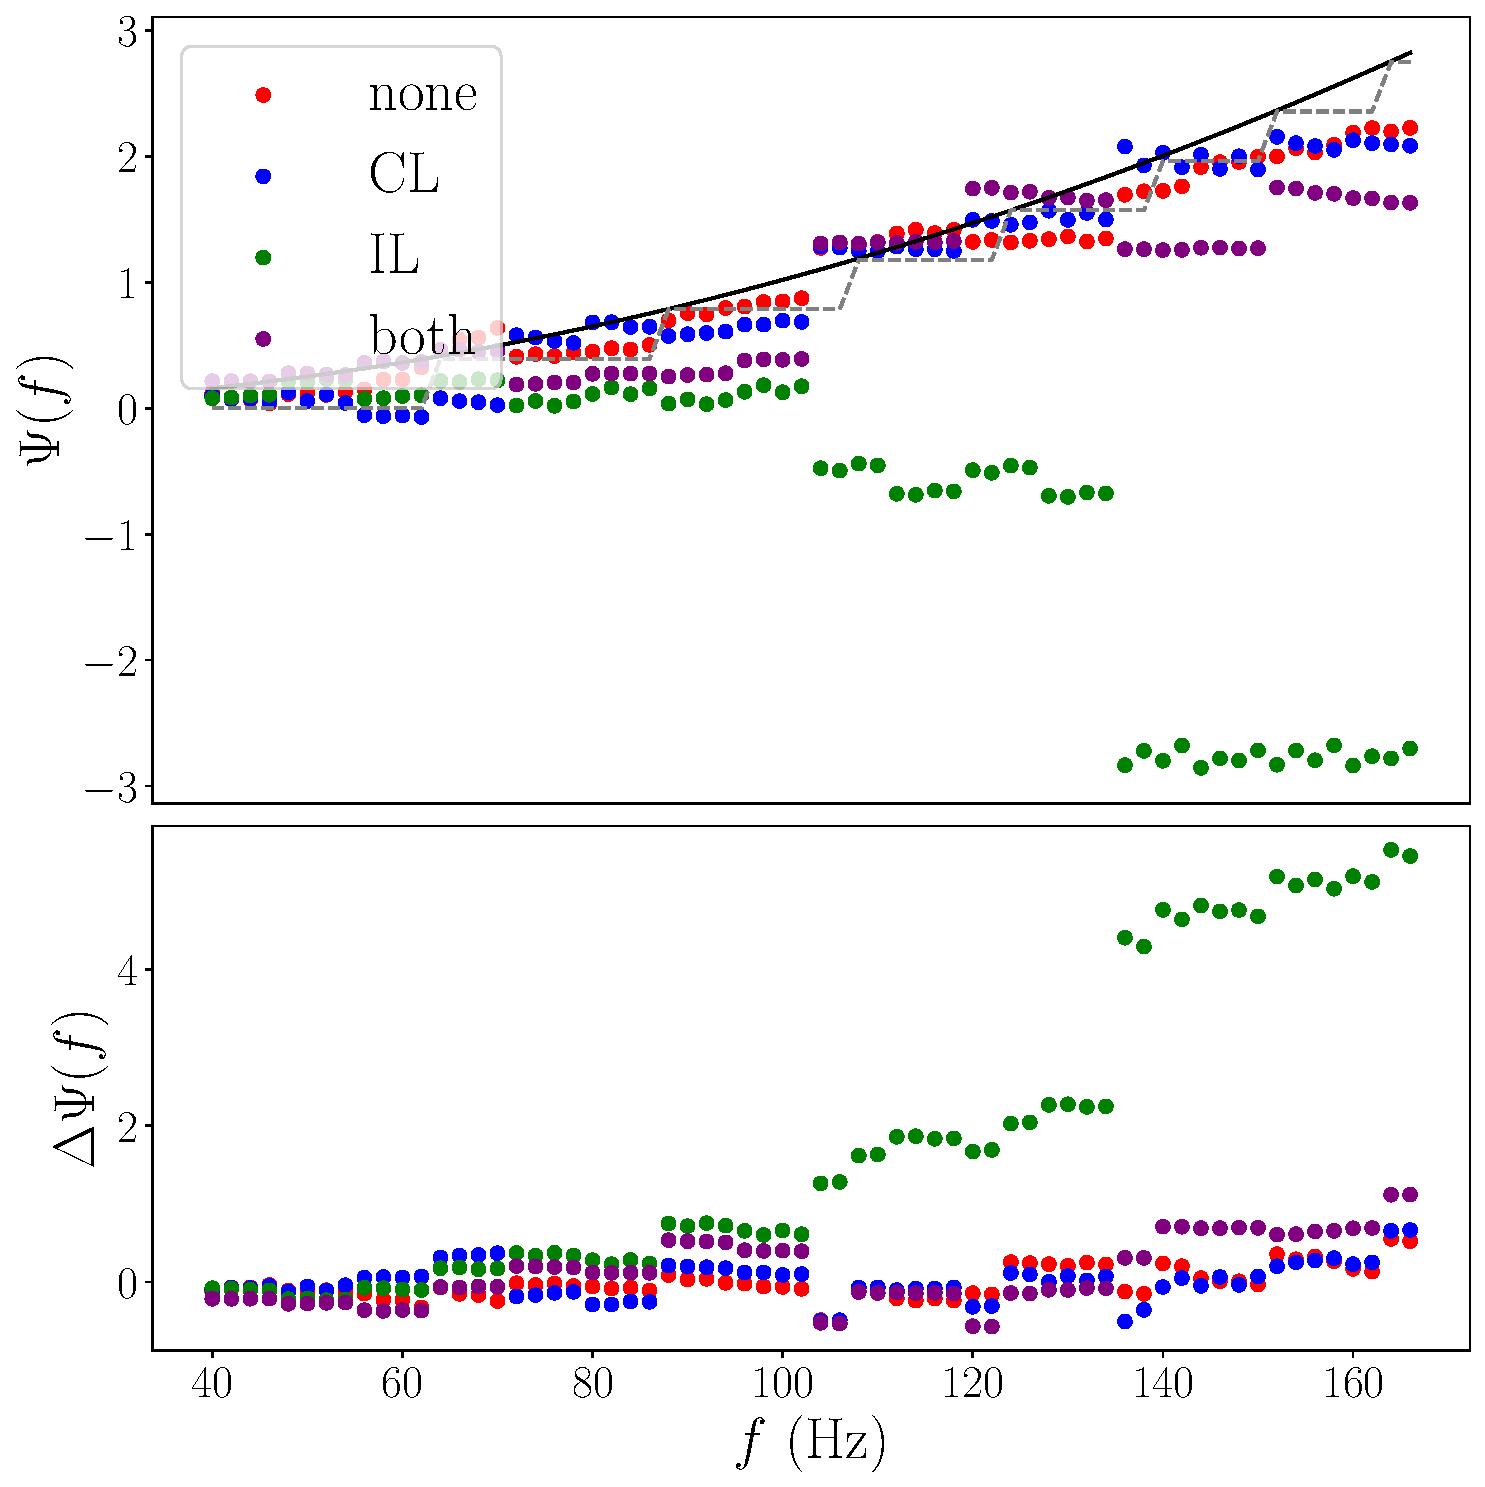
\includegraphics[width=\textwidth]{im/phase_RP_comp_quadratic_m4}
\caption{Effects of fixing parameters for $\Psi(f) \sim f^2$ ($L=6$, $m=4$, 600 epochs, SAM)}
\end{figure}
\end{column}
\end{columns}
\end{frame}

\begin{frame}
\frametitle{Fixing Parameters}
\begin{itemize}
\item Legend for the plots on the previous slide:
\begin{itemize}
\item `\emph{none}' : no parameters fixed 
\item `\emph{CL}': only CL parameters fixed
\item `\emph{IL}': only IL parameters fixed 
\item `\emph{both}': all parameters fixed  
\end{itemize} 
\item Evidently, keeping parameters fixed leads to  \alert{worse performance}, likely due to a reduction of the search space  
\item Note that fixing parameters leads to high $\epsilon$ and hence potentially somewhat meaningless results 
\item Thus, especially taking into account the equivalent computational times, \alert{not keeping parameters fixed yields better results} 
\item Notably `\emph{IL}' results in worse performance than `\emph{CL}',  suggesting a particular importance of ILs compared to CLs 
\end{itemize}
\end{frame}

\section{Improving the Loss Function}

\begin{frame}
\frametitle{Formalisation}
\begin{itemize}
\item Consider a computational basis state, $\ket{k}$, of the \alert{combined} input-register-target-register \alert{system} 
\item The state $\ket{k}$ is associated with a \alert{bit string} $k = \{0,1 \}^{n+m}$
\item Denote by $[k]_n$ and $[k]_m$ the bit strings of length $n$ and $m$, respectively, associated with each of the registers and write their \alert{concatenation} as 
\begin{equation}
k \equiv [k]_n \diamond [k]_m
\end{equation} 
\item A general state of the two-register system is then written as 
\begin{equation}
\ket{z} = \sum^{2^{n+m}-1}_{k=0} z_k \ket{k}
\end{equation}
and referred to via its \alert{coefficients} $z_k$
\end{itemize}
\end{frame}

\begin{frame}
\frametitle{Formalisation}
\begin{itemize}
\item When training in superposition, the \alert{desired state} of the system is 
\begin{equation}
\ket{y} = \sum_{j=0}^{2^n-1} \frac{1}{\sqrt{2^n}} \ket{j}_i \ket{\Psi(j)}_t,
\end{equation}
where the subscripts $i$ and $t$ indicate basis states of the input and target registers, respectively
\item This state $\ket{y}$ can be written in terms of the \alert{combined basis} $\{ \ket{k} \}$ via 
\begin{equation}
y_k = \begin{cases}
\frac{1}{\sqrt{2^n}}  & \text{if } k=[k]_n \diamond \Psi([k]_n) \\
0 & \text{else} 
\end{cases}
\end{equation}
\item Further denote the \alert{output state} produced by the QCNN by $\ket{x}$, with associated coefficients $x_k$
\end{itemize}
\end{frame}

\begin{frame}
\frametitle{SAM and Beyond}
\begin{itemize}
\item Recall the definition of \alert{SAM}:
\begin{equation}
\text{SAM}(\ket{x}, \ket{y}) = 1 - \sum_k |x_k| | y_k |  
\end{equation}
\item By construction, this is closely related to the \alert{mismatch} 
\begin{equation}
\mathsf{M}(\ket{x}, \ket{y}) = 1 - \left|\sum_k x_k y_k\right|
\end{equation}
\item While effective, SAM's \alert{fundamental flaw} is that it does not directly take into account the amplitudes $x_k$ for $k$ where $y_k =0$ (i.e. where $[k]_m \neq \Psi([k]_n)$
\end{itemize}
\end{frame}

\begin{frame}
\frametitle{SAM and Beyond}
\begin{itemize}
\item Consider $k=a$ and $k=b$ with $[k]_m \neq \Psi([k]_n)$ for both and 
\begin{equation}
\Big|[a]_m - \Psi([a]_n) \Big| > \Big|[b]_m - \Psi([b]_n) \Big| 
\end{equation}
\item To improve performance, the loss function should punish a non-zero $x_a$ more than a non-zero $x_b$ which is not the case for SAM
\item This could be achieved via a \alert{weighted mismatch (WIM)}, 
\begin{equation}
\text{WIM}(\ket{x}, \ket{y}) =  1 - \sum_k \tilde{w}_k |x_k| |y_k |, 
\end{equation}
where $\tilde{w}_k \in \mathbb{R}_+$ are appropriate weights
\end{itemize}
\end{frame}

\begin{frame}
\frametitle{SAM and Beyond}
\begin{itemize}
\item It was discussed at the last meeting to base the weights on
\begin{equation}
w_k = \sum^{2^m -1}_{\substack{l=0, \\ l \neq [k]_m}} \Big|x_{[k]_n \diamond l} \Big| \Big| l - \Psi([k]_n) \Big|,
\end{equation}
with the $\tilde{w}_k$ obtained from the $w_k$ via normalisation and smoothing
\item Implementing this \alert{proved to be ineffective}, with no improvement on SAM  (see later)
\item This raises broader questions about the \alert{feasibility of WIM}: is adding weights sufficient to alter SAM's fundamental dynamic of neglecting $x_k$ for $k$ with $y_k =0$?
\end{itemize}
\end{frame}

\begin{frame}
\frametitle{Introducing WILL}
\begin{itemize}
\item To improve on SAM, it could instead be beneficial to return to a loss function which more directly takes into account all $x_k$ 
\item Define \alert{L$_\text{p}$ loss} as 
\begin{equation}
\text{LL}_\text{p} (\ket{x}, \ket{y}) = \left( \sum_k |x_k -y_k|^p \right)^{1/p}
\end{equation}
\item As discussed, \alert{computational basis states are not equidistant} for phase encoding: their distance depends on the value they encode on the input and target registers
\item A \alert{weighted L$_\text{p}$ loss (WILL)} can factor in an appropriate distance measure for the state space:
\begin{equation}
\text{WILL}_\text{p,q} =  \left( \sum_k \Big|x_k -y_k \Big|^p \Big|[k]_m - \Psi([k]_n) \Big|^q \right)^{1/p}
\end{equation}
\end{itemize}
\end{frame}

\begin{frame}
\frametitle{Testing WILL}
\begin{columns}
\begin{column}{0.5\textwidth}
\begin{figure}
\centering 
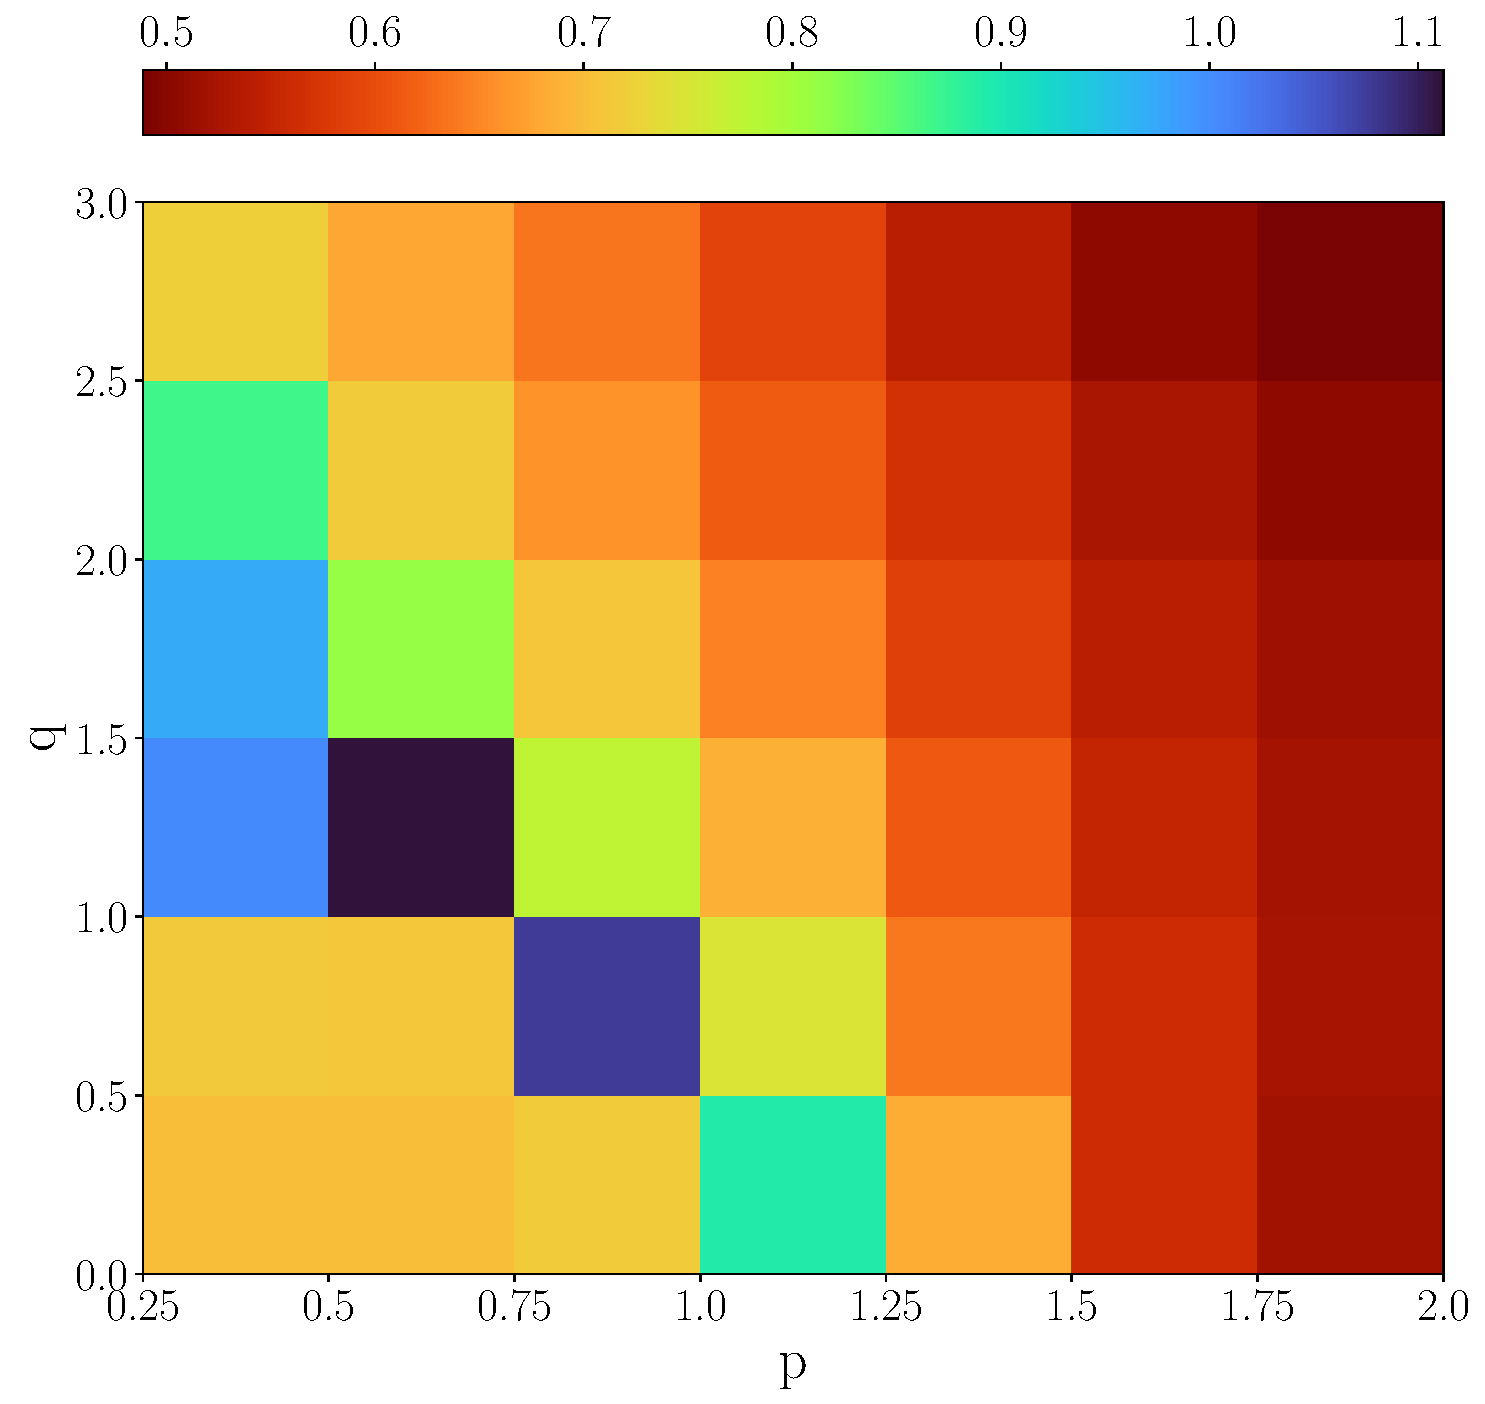
\includegraphics[width=\textwidth]{im/omega_3_6_600_linear}
\caption{Comparing $\Omega$ for various $p$, $q$ ($L=6$, $m=3$, 600 epochs, $\Psi(f)\sim f$)}
\end{figure}
\end{column}
\begin{column}{0.5\textwidth}
\begin{figure}
\centering 
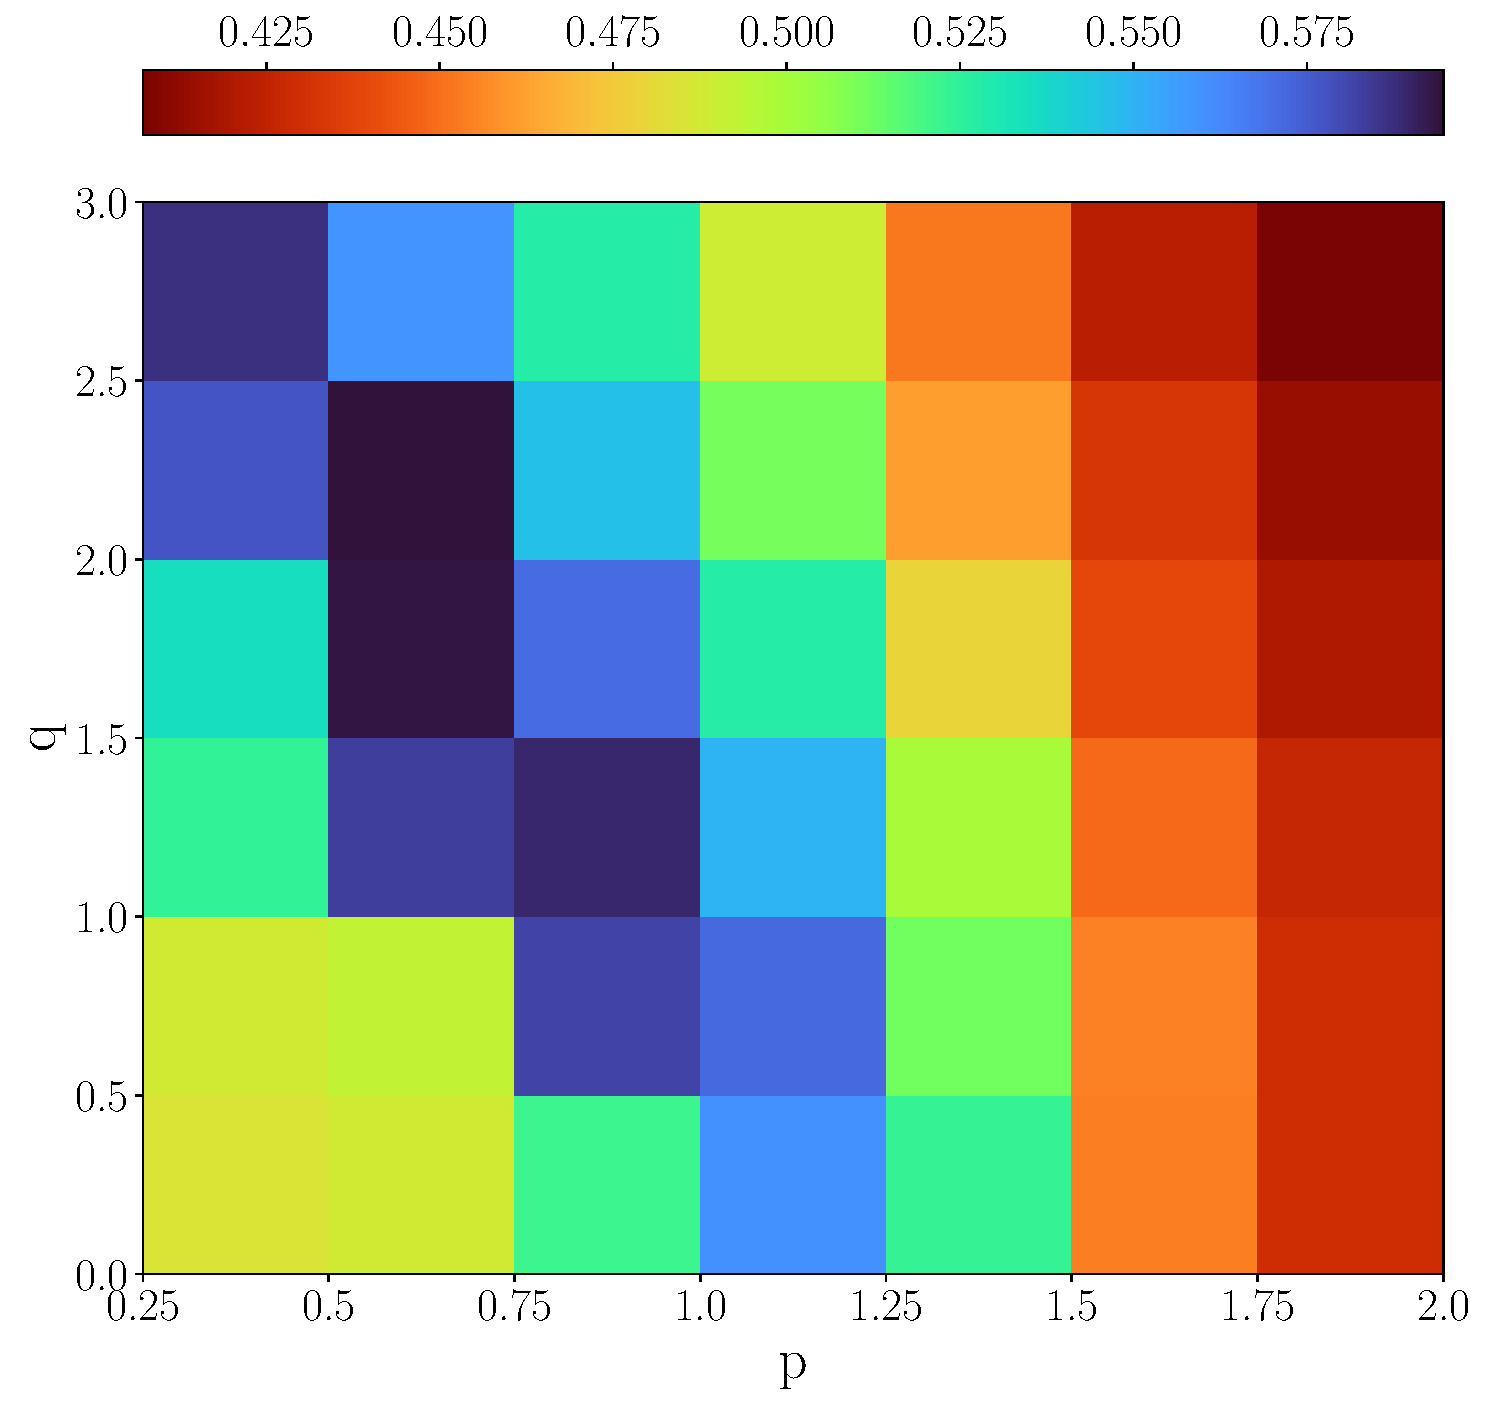
\includegraphics[width=\textwidth]{im/omega_3_6_600_quadratic}
\caption{Comparing $\Omega$ for various $p$, $q$ ($L=6$, $m=3$, 600 epochs, $\Psi(f)\sim f^2$)}
\end{figure}
\end{column}
\end{columns}
\end{frame}

\begin{frame}
\frametitle{Comparing SAM, WIM, and WILL}
\begin{columns}
\begin{column}{0.5\textwidth}
\begin{table}
\begin{tabular}{c || c| c| c }
& SAM & WIM & WILL \\ \hline \hline 
$\mu$ &  \textbf{3.4e-2} & 6.0e-2 & 3.0e-1 \\
$\sigma$ &  1.4e-1 &1.1e-1 & \textbf{ 1.7e-2}\\
$\epsilon$  &  \textbf{1.9e-2} & 9.2e-2 & 1.9e-1\\
$\chi$ & \textbf{ 3.2e-2} & 5.1e-2  & 3.9e-1  \\ \hline 
$\Omega$ &  \textbf{4.46} & 3.19 & 1.11
\end{tabular}
\caption{Comparing loss function metrics for $\Psi(f) \sim f$ ($L=6$, $m=3$, 600 epochs)}
\end{table}
\end{column}
\begin{column}{0.5\textwidth}
\begin{figure}
\centering 
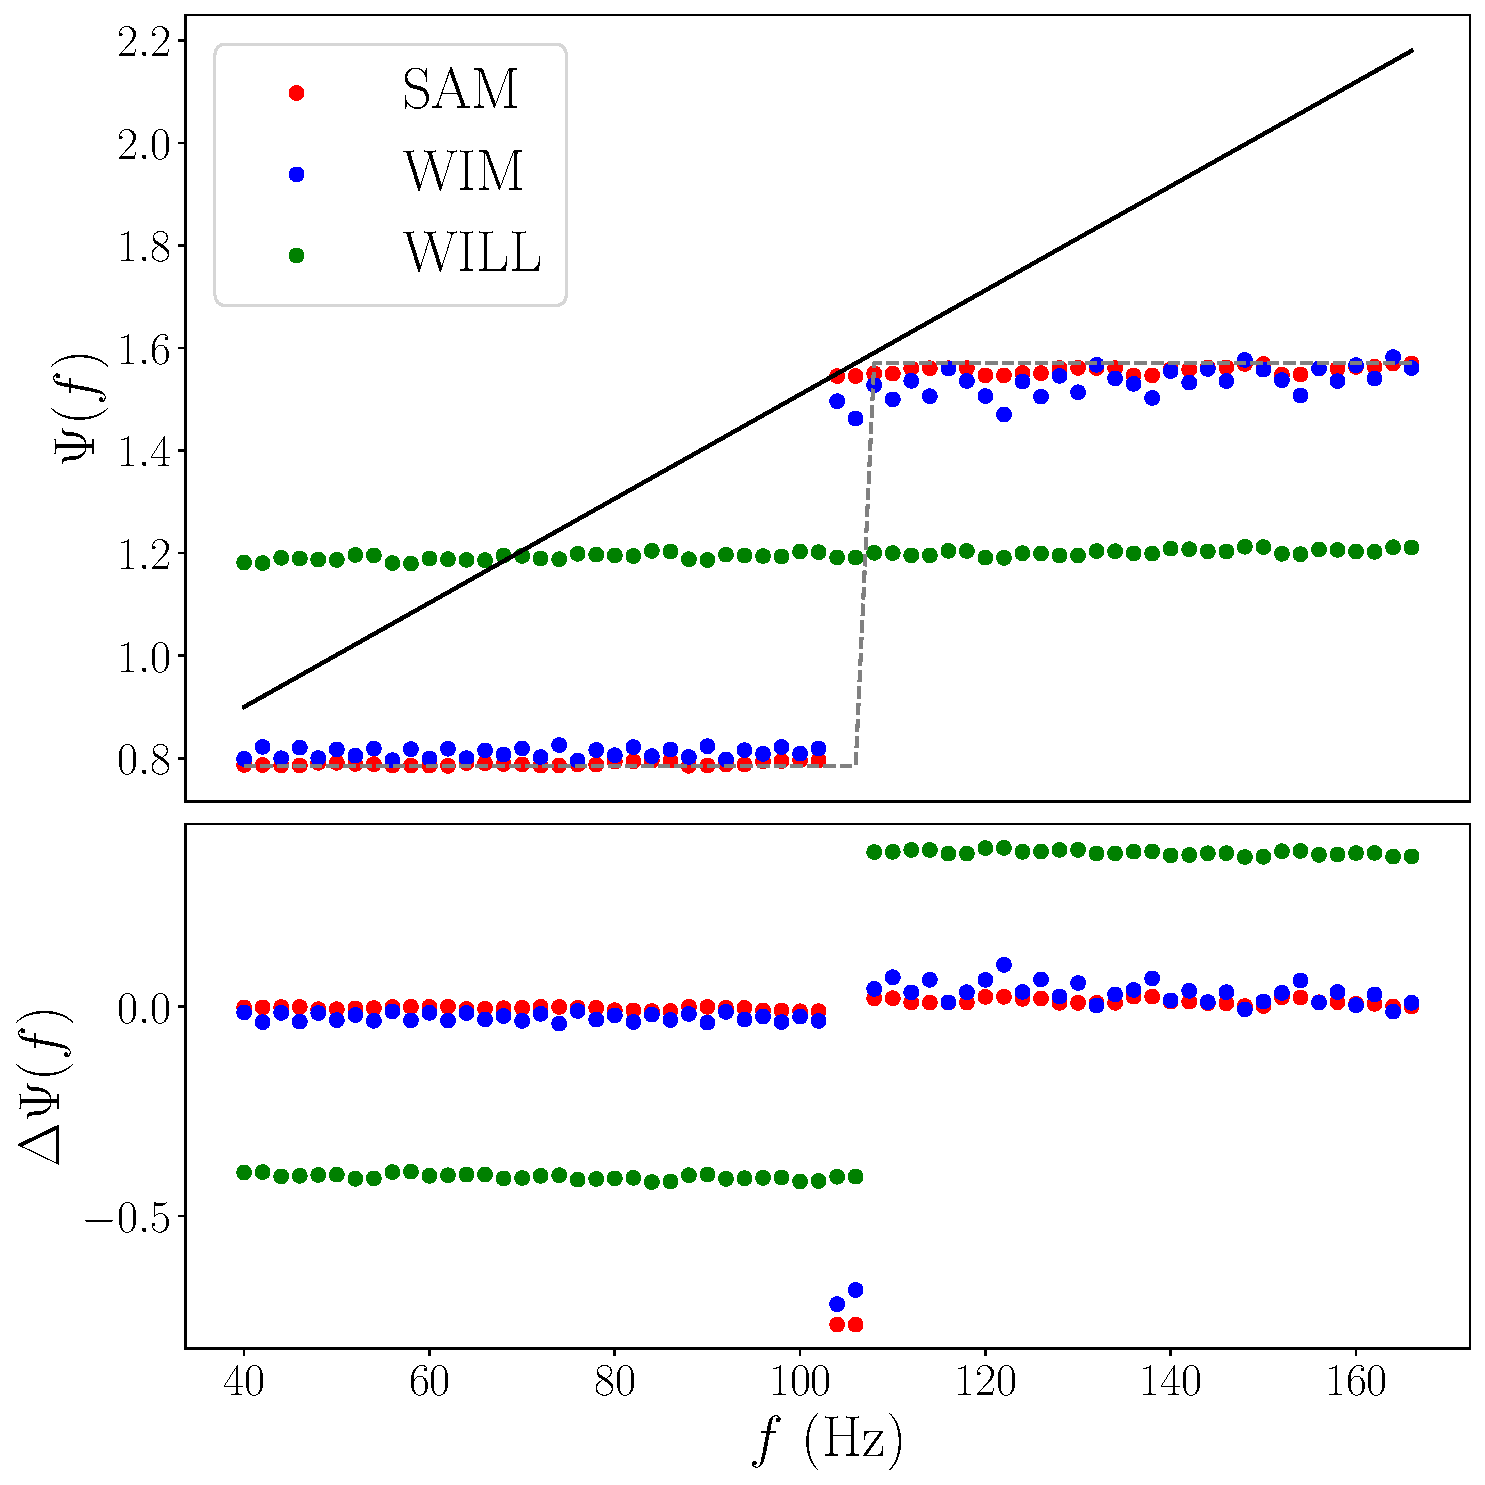
\includegraphics[width=\textwidth]{im/SAM_WIM_WILL_F}
\caption{Comparing extracted phase functions for $\Psi(f) \sim f$ ($L=6$, $m=3$, 600 epochs)}
\end{figure}
\end{column}
\end{columns}
\end{frame}

\begin{frame}
\frametitle{Comparing SAM, WIM, and WILL}
\begin{columns}
\begin{column}{0.5\textwidth}
\begin{table}
\begin{tabular}{c || c| c| c }
& SAM & WIM & WILL \\ \hline \hline 
$\mu$ &  \textbf{1.9e-1} & 2.3e-1 & 4.7e-1 \\
$\sigma$ &  1.2e-1 & \textbf{1.0e-1} & 1.5e-1\\
$\epsilon$  &  \textbf{2.2e-1} & 4.2e-1 & 3.8e-1\\
$\chi$ &  \textbf{1.9e-1} & 2.0e-1 & 6.8e-1 \\ \hline 
$\Omega$ &  \textbf{1.39} & 1.05 & 0.60
\end{tabular}
\caption{Comparing loss function metrics for $\Psi(f) \sim f^2$ ($L=6$, $m=3$, 600 epochs)}
\end{table}
\end{column}
\begin{column}{0.5\textwidth}
\begin{figure}
\centering 
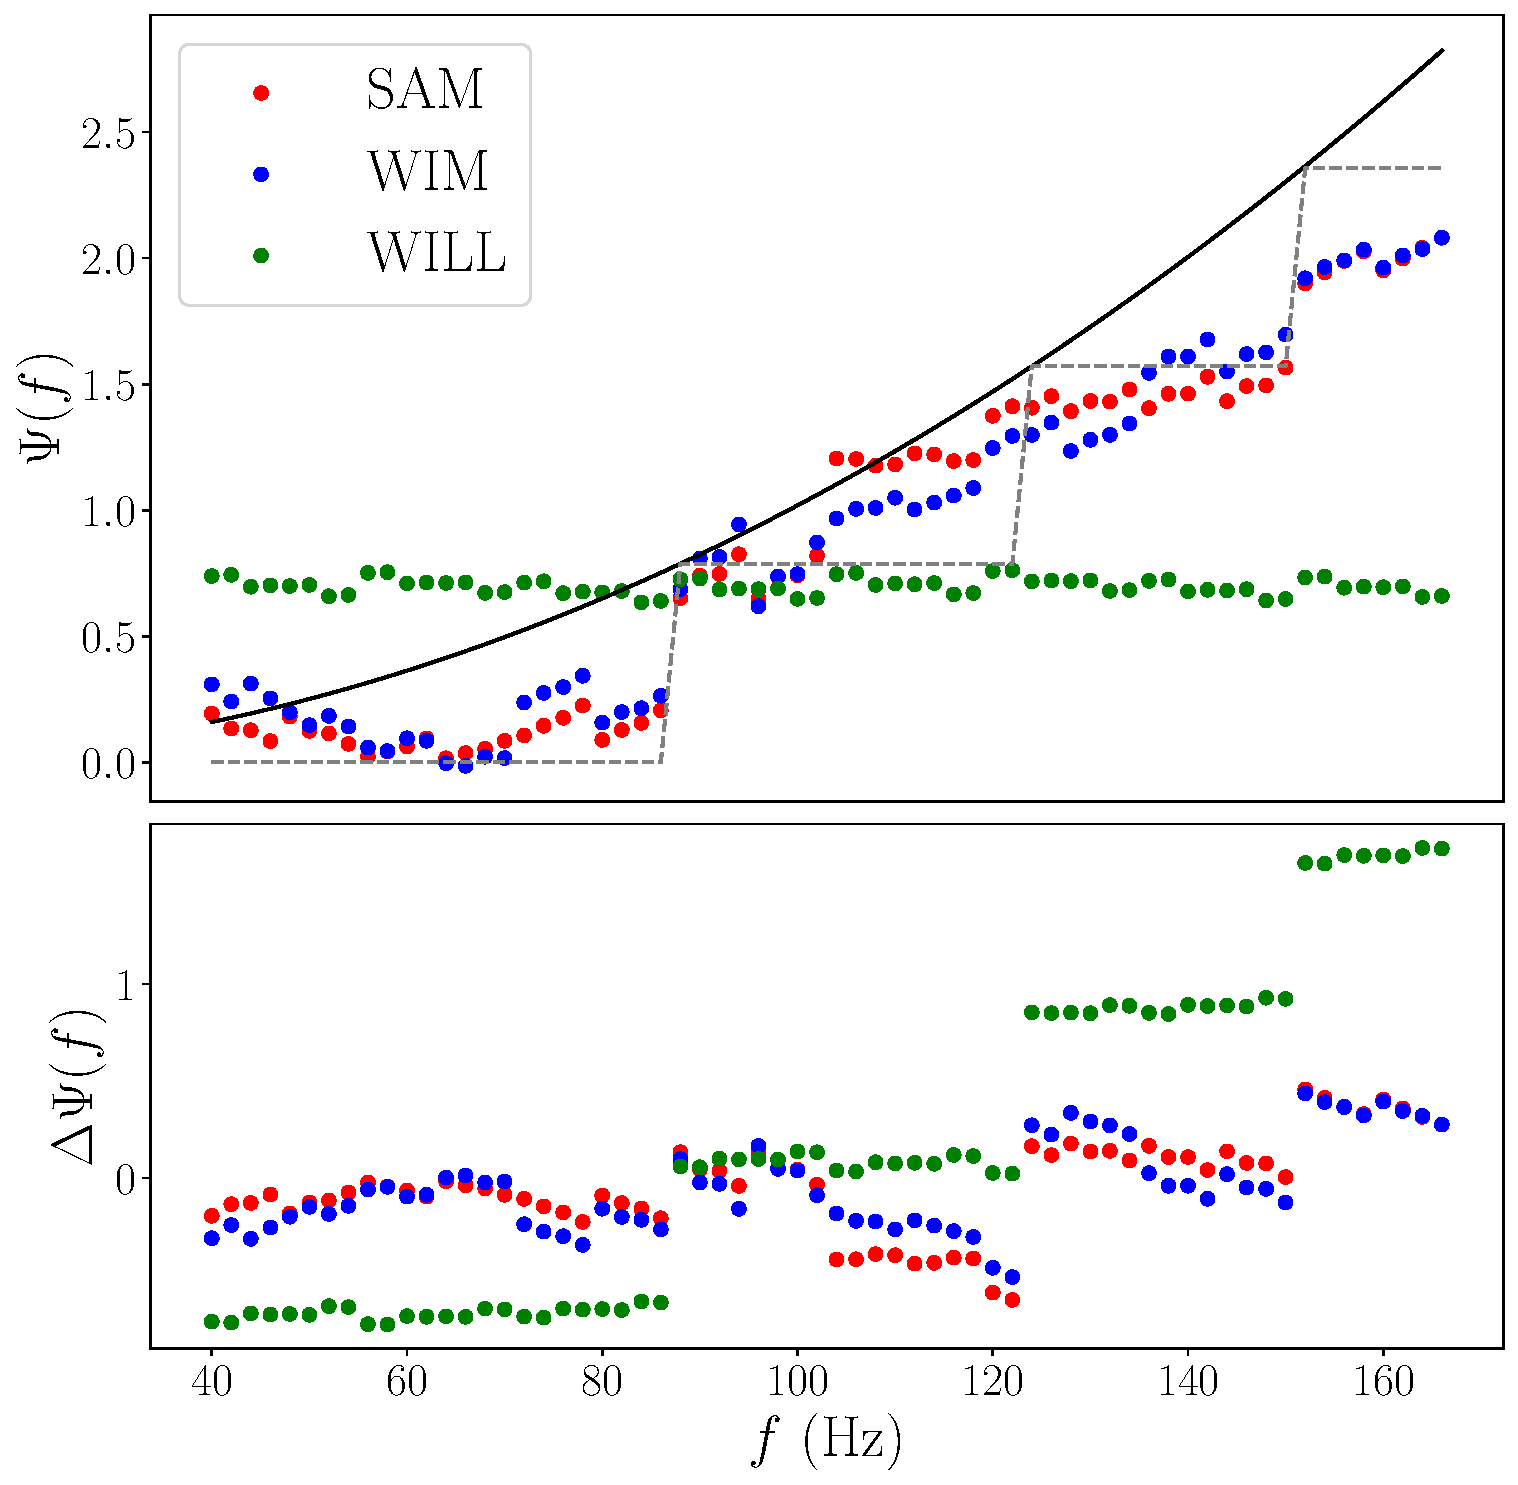
\includegraphics[width=\textwidth]{im/SAM_WIM_WILL_F2}
\caption{Comparing extracted phase functions for $\Psi(f) \sim f^2$ ($L=6$, $m=3$, 600 epochs)}
\end{figure}
\end{column}
\end{columns}
\end{frame}

\begin{frame}
\frametitle{Comparing SAM, WIM, and WILL}
\begin{columns}
\begin{column}{0.5\textwidth}
\begin{table}
\begin{tabular}{c || c| c| c }
& SAM & WIM & WILL \\ \hline \hline 
$\mu$ &  \textbf{6.8e-2} & 8.4e-2 & 7.1e-2 \\
$\sigma$ &  1.8e-1 & \textbf{1.2e-1} & 2.1e-1\\
$\epsilon$  &  4.5e-2 & 1.8e-1 & \textbf{2.7e-2}\\
$\chi$ &  7.4e-2 & 1.0e-1 & \textbf{7.0e-2} \\ \hline 
$\Omega$ &  \textbf{2.75} & 2.07 & 2.63
\end{tabular}
\caption{Comparing loss function metrics for $\Psi_\text{H23}$ ($L=6$, $m=3$, 600 epochs)}
\end{table}
\end{column}
\begin{column}{0.5\textwidth}
\begin{figure}
\centering 
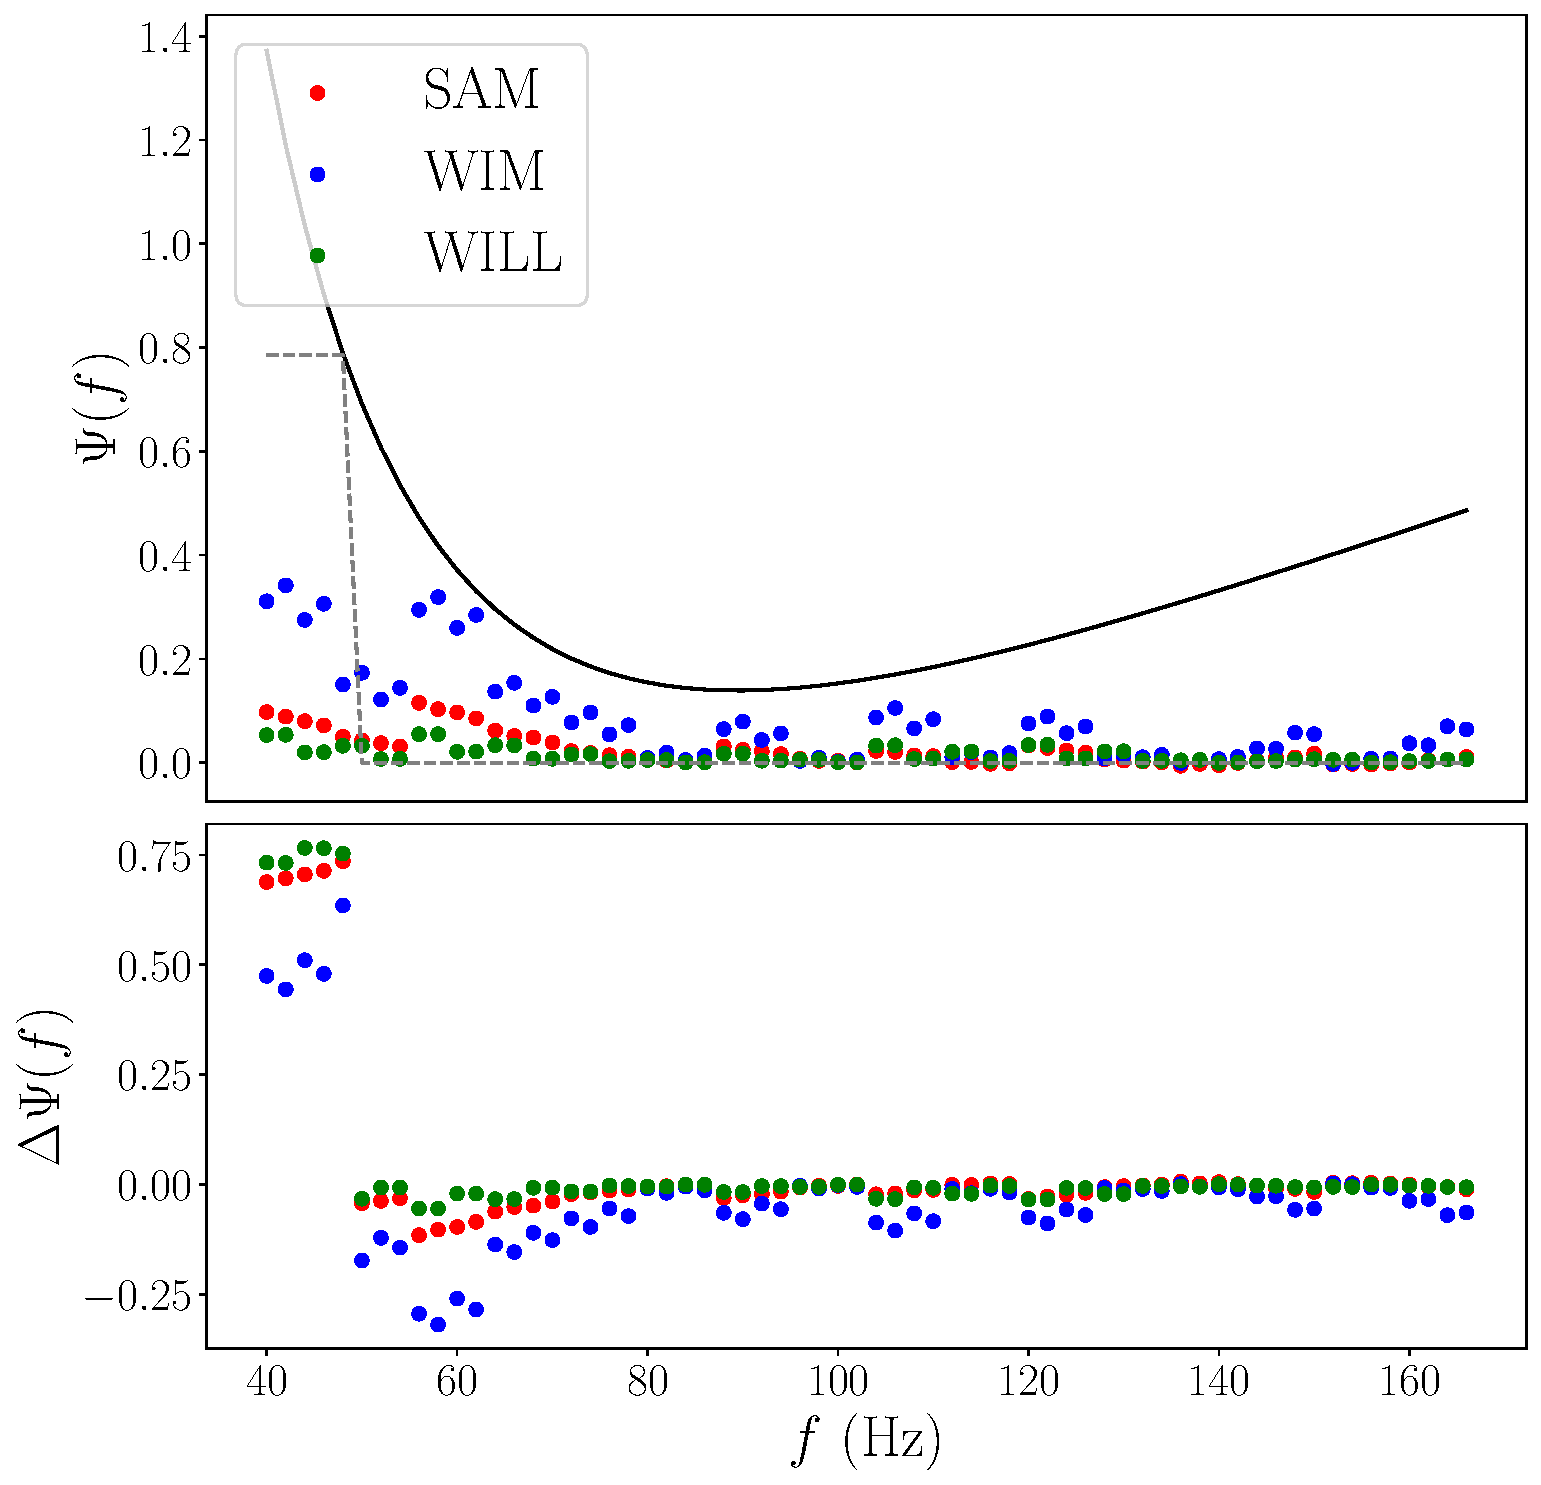
\includegraphics[width=\textwidth]{im/SAM_WIM_WILL_H}
\caption{Comparing extracted phase functions for $\Psi_\text{H23}$ ($L=6$, $m=3$, 600 epochs)}
\end{figure}
\end{column}
\end{columns}
\end{frame}

\begin{frame}
\frametitle{Loss Function Conclusion}
\begin{itemize}
\item The attempts to improve upon SAM via \alert{WIM and WILL have failed}\footnote{A fix in the definition of WILL could potentially change this!} 
\item No further \emph{ansatz} to design a new loss function could be identified
\item Further \alert{QCNN improvements} might have to come from something \alert{other than the loss function} 
\end{itemize}
\end{frame}

\section{Exploring Correlations}

\begin{frame}
\frametitle{Exploring Correlations}
\begin{itemize}
\item The following investigates \alert{correlations between the metrics} $\mu$, $\sigma$, $\chi$, and $\epsilon$ in an attempt to better understand the relationship between phase extraction and $\hat{Q}_\Psi$
\item This is done by analysing the outputs of $N=267$ different QCNNs with \alert{various different configurations} (i.e. $L$, $m$, loss functions, $\Psi$,...)
\item Key questions to answer are:
\begin{itemize}
\item Is a low normalisation error $\epsilon$ an indicator of a good fit, i.e. low $\chi$?
\item Is a low mean mismatch $\mu$ a guarantee of low $\epsilon$, $\chi$? 
\item What is the role of $\sigma$?
\end{itemize}
\end{itemize}
\end{frame}

\begin{frame}
\frametitle{Exploring Correlations}
\begin{columns}
\begin{column}{0.5\textwidth}
\begin{figure}
\centering 
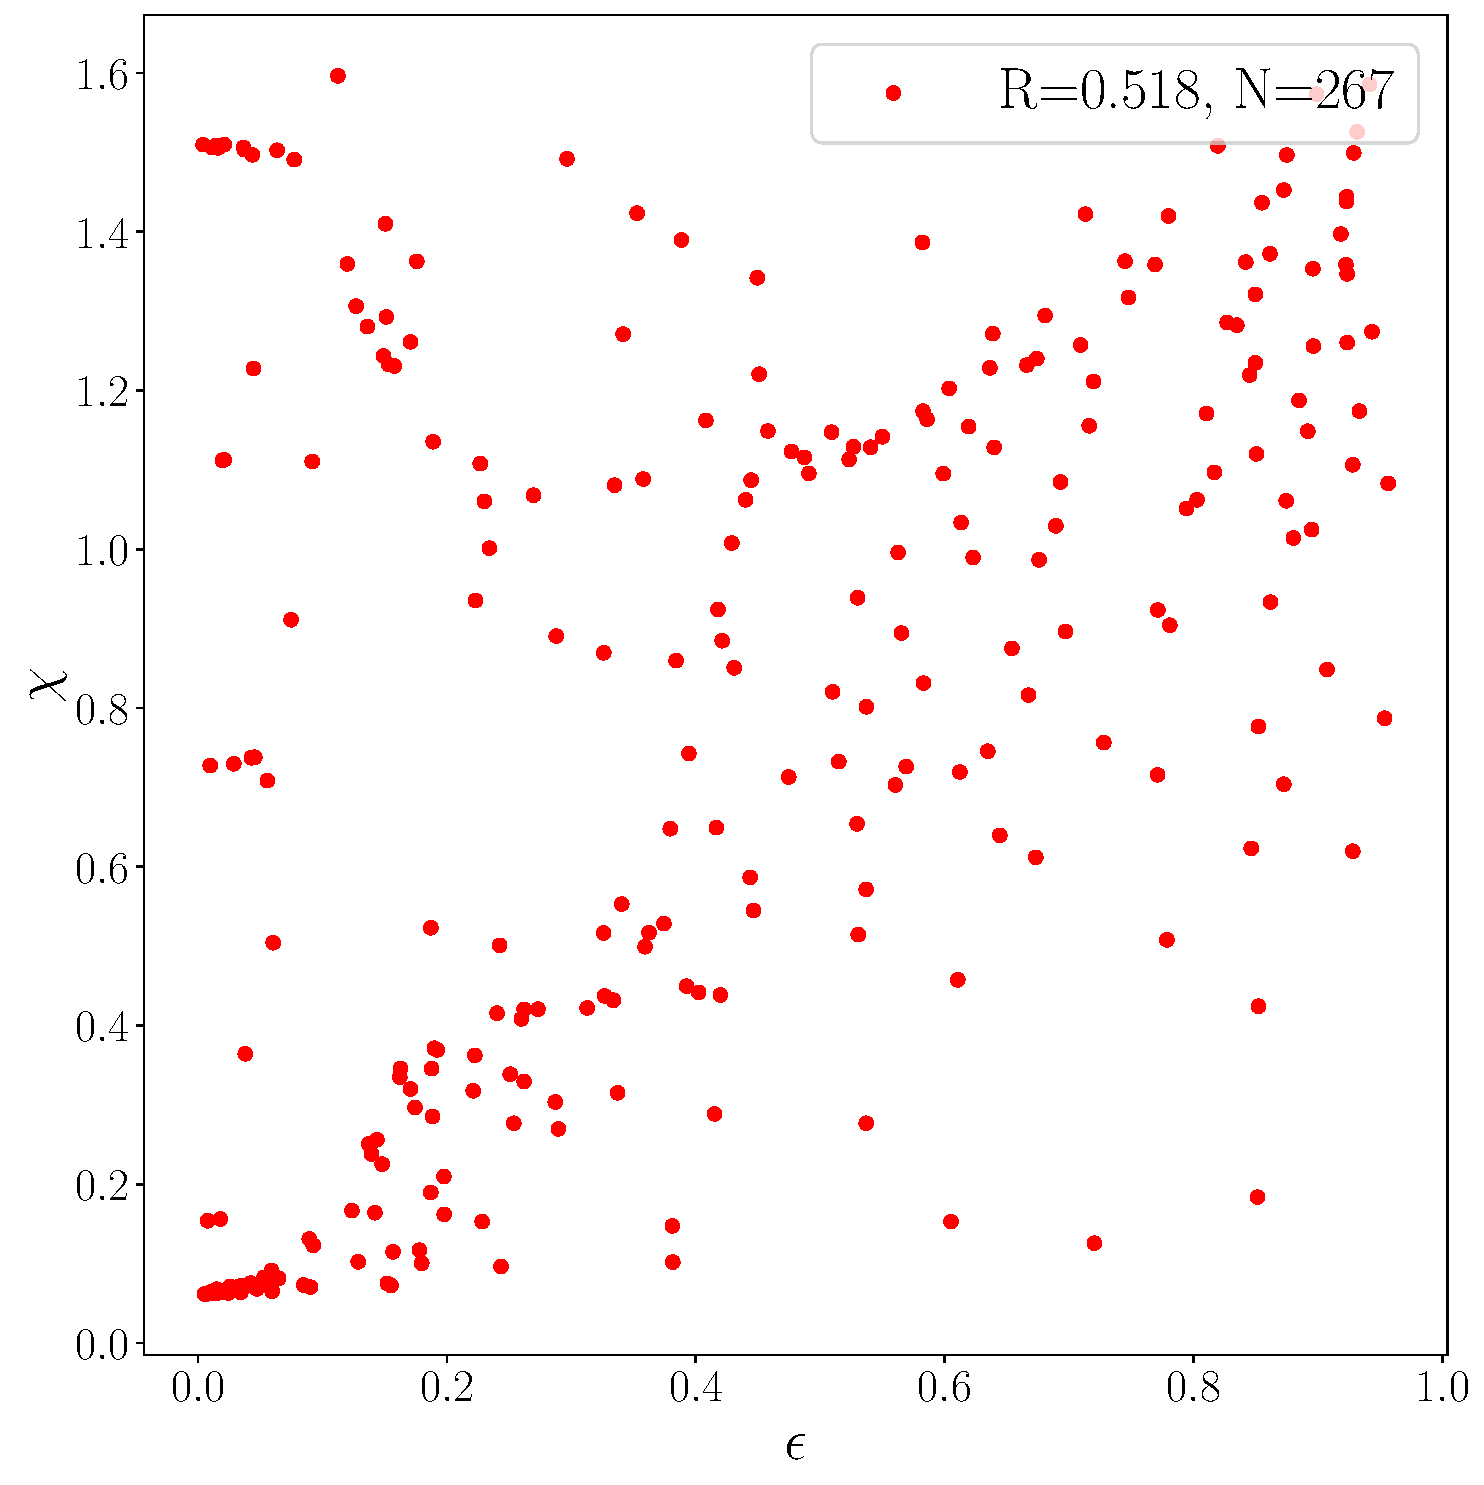
\includegraphics[width=\textwidth]{im/eps_v_chi_}
\caption{Correlation between $\epsilon$ and $\chi$.}
\end{figure}
\end{column}
\begin{column}{0.5\textwidth}
\begin{figure}
\centering 
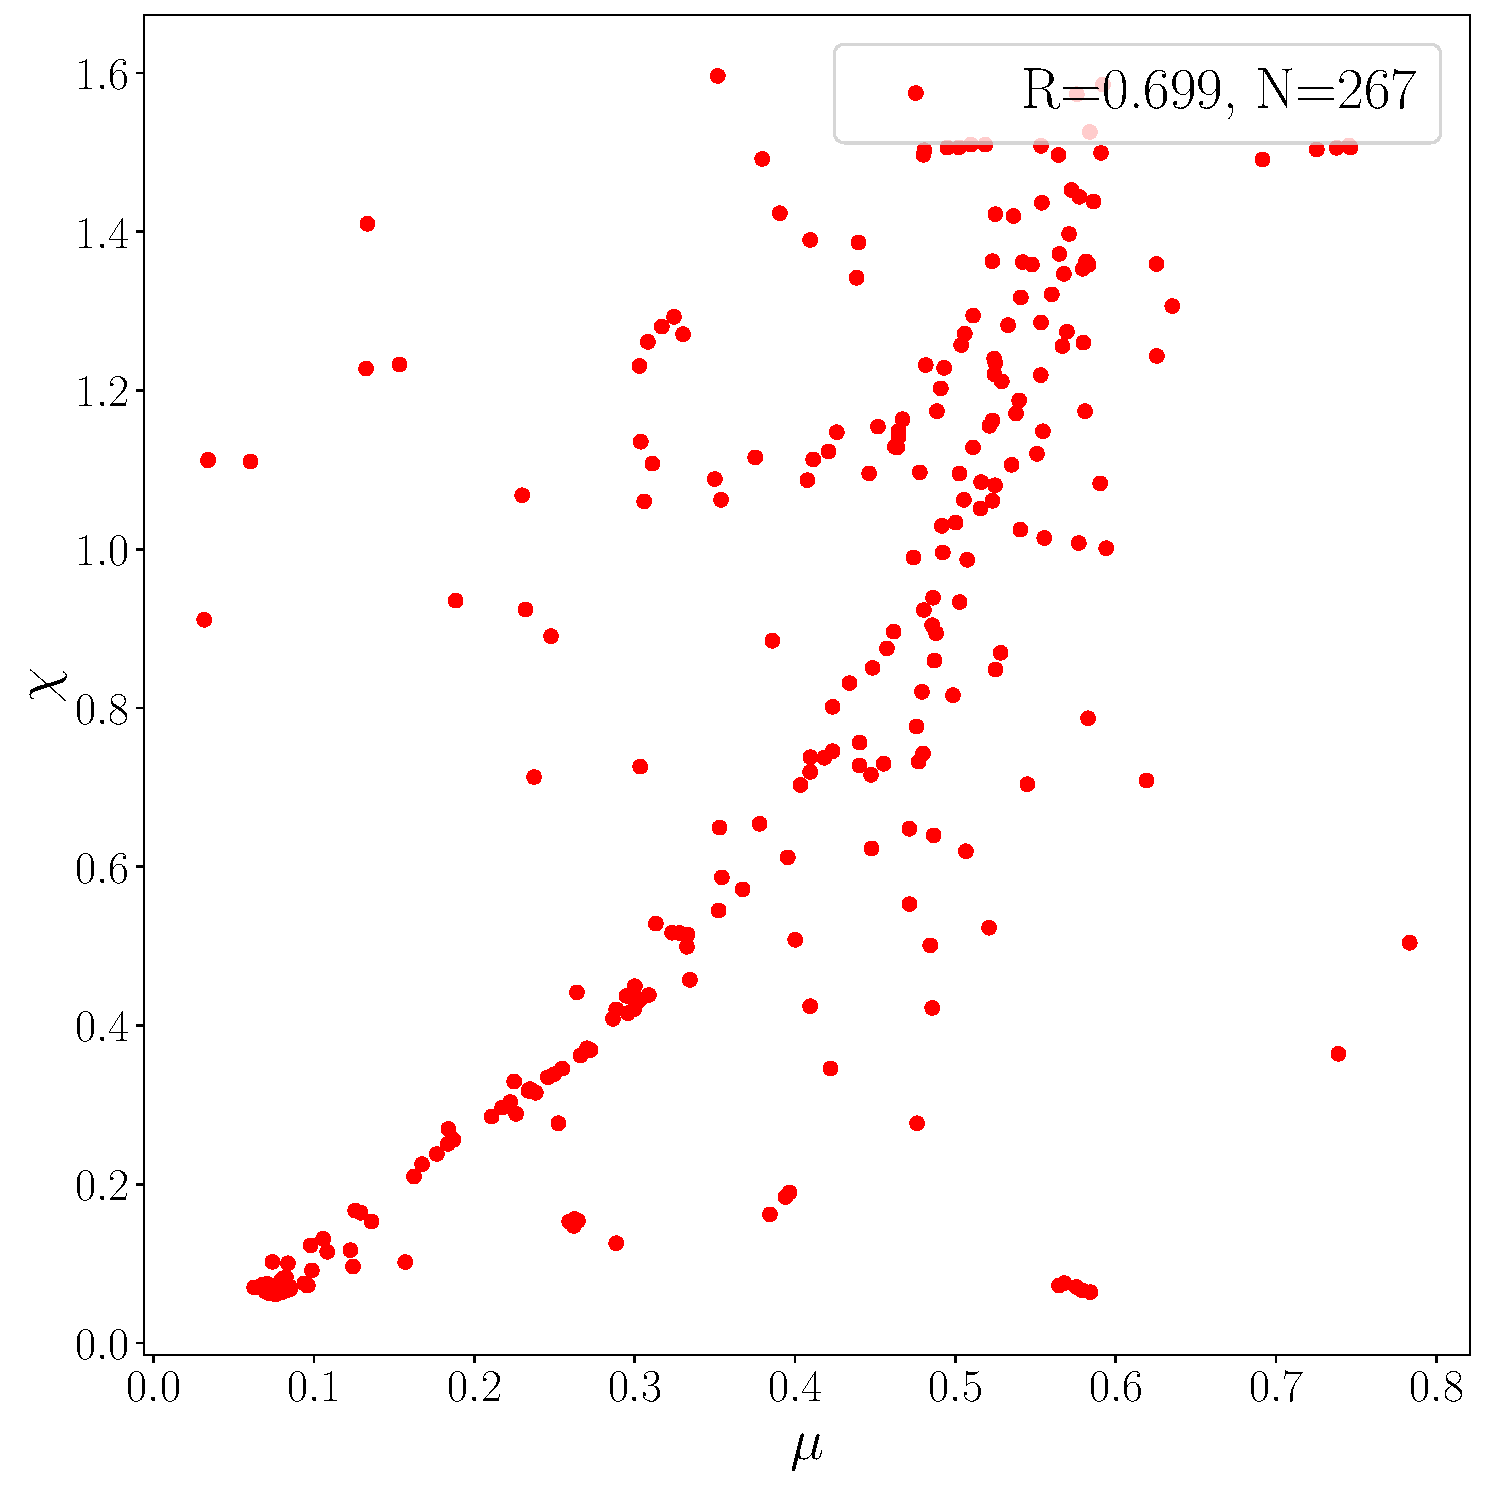
\includegraphics[width=\textwidth]{im/mu_v_chi_}
\caption{Correlation between $\mu$ and $\chi$.}
\end{figure}
\end{column}
\end{columns}
\end{frame}

\begin{frame}
\frametitle{Exploring Correlations}
\begin{columns}
\begin{column}{0.5\textwidth}
\begin{figure}
\centering 
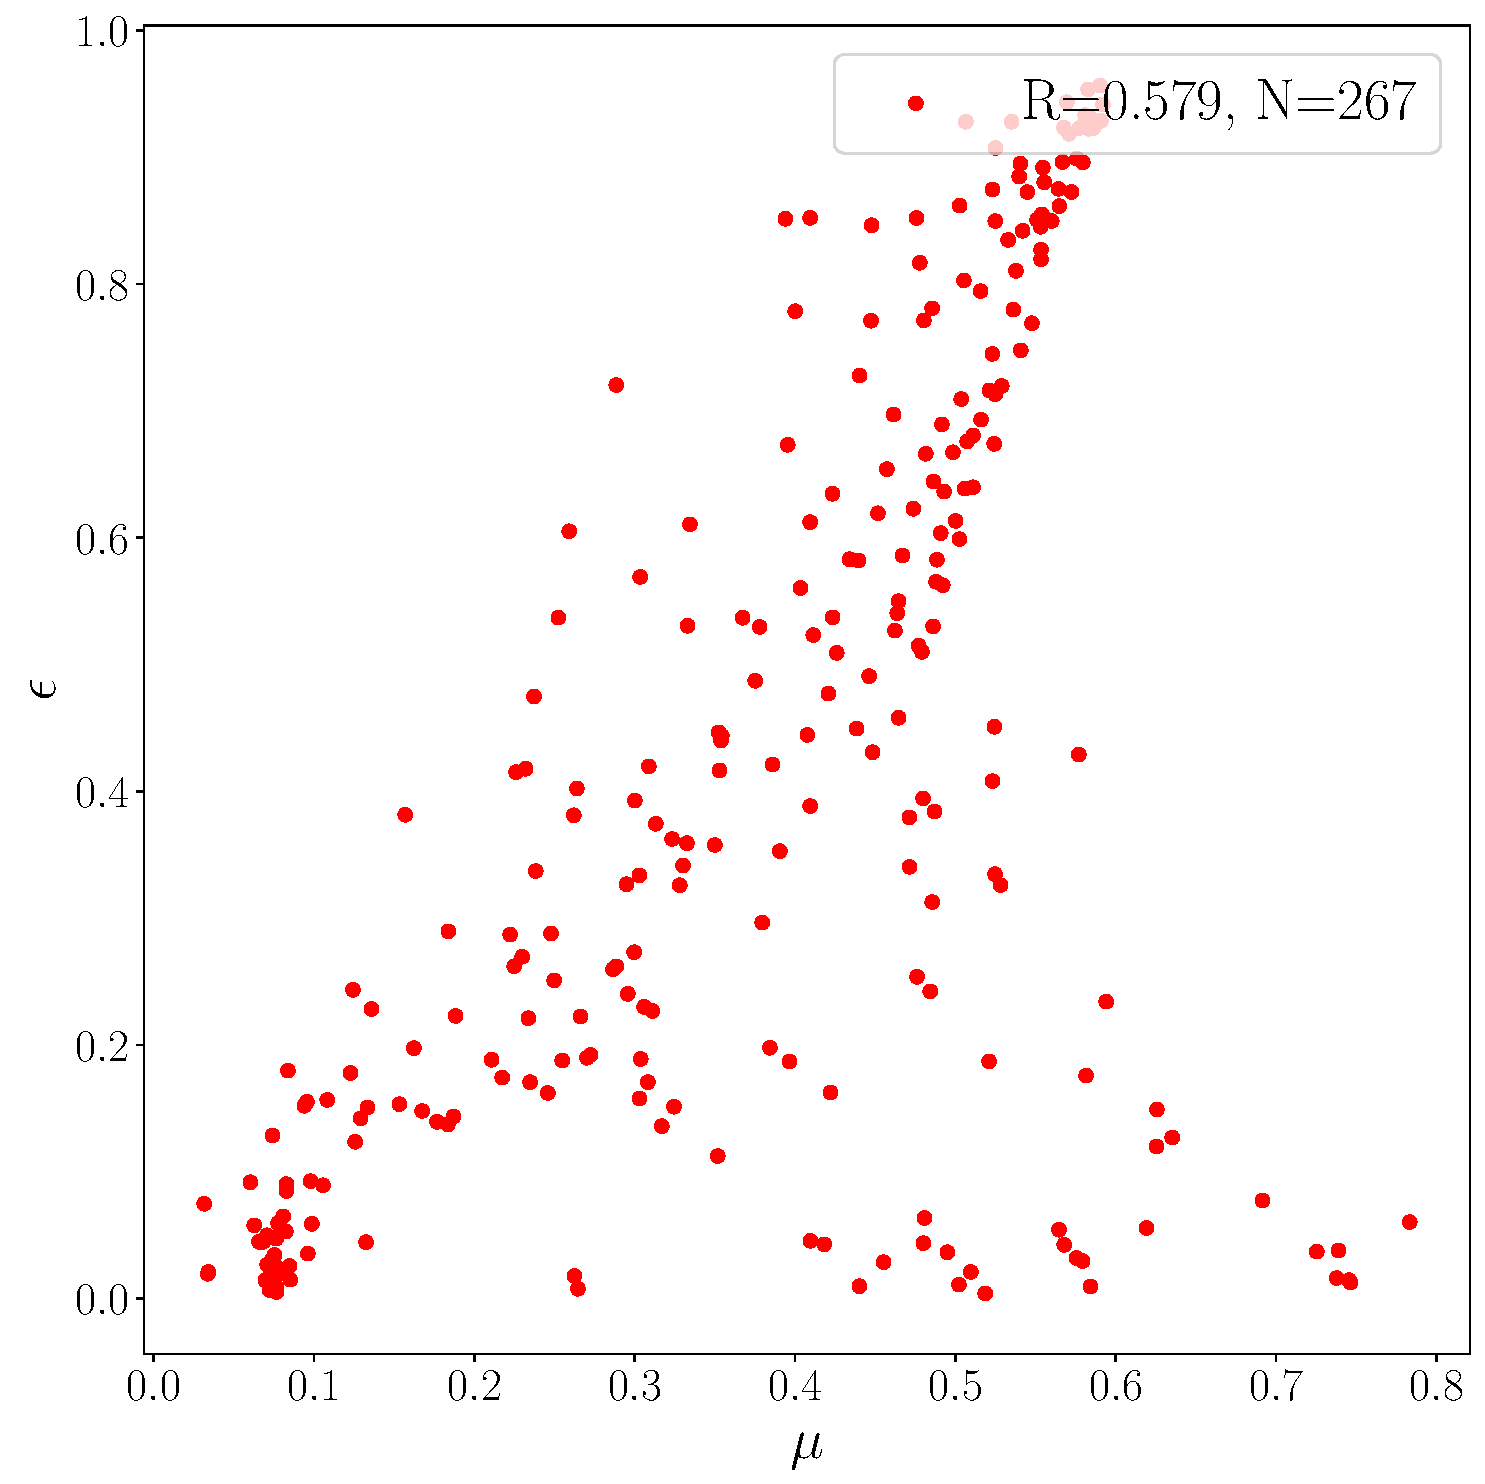
\includegraphics[width=\textwidth]{im/mu_v_eps_}
\caption{Correlation between $\mu$ and $\epsilon$.}
\end{figure}
\end{column}
\begin{column}{0.5\textwidth}
\begin{figure}
\centering 
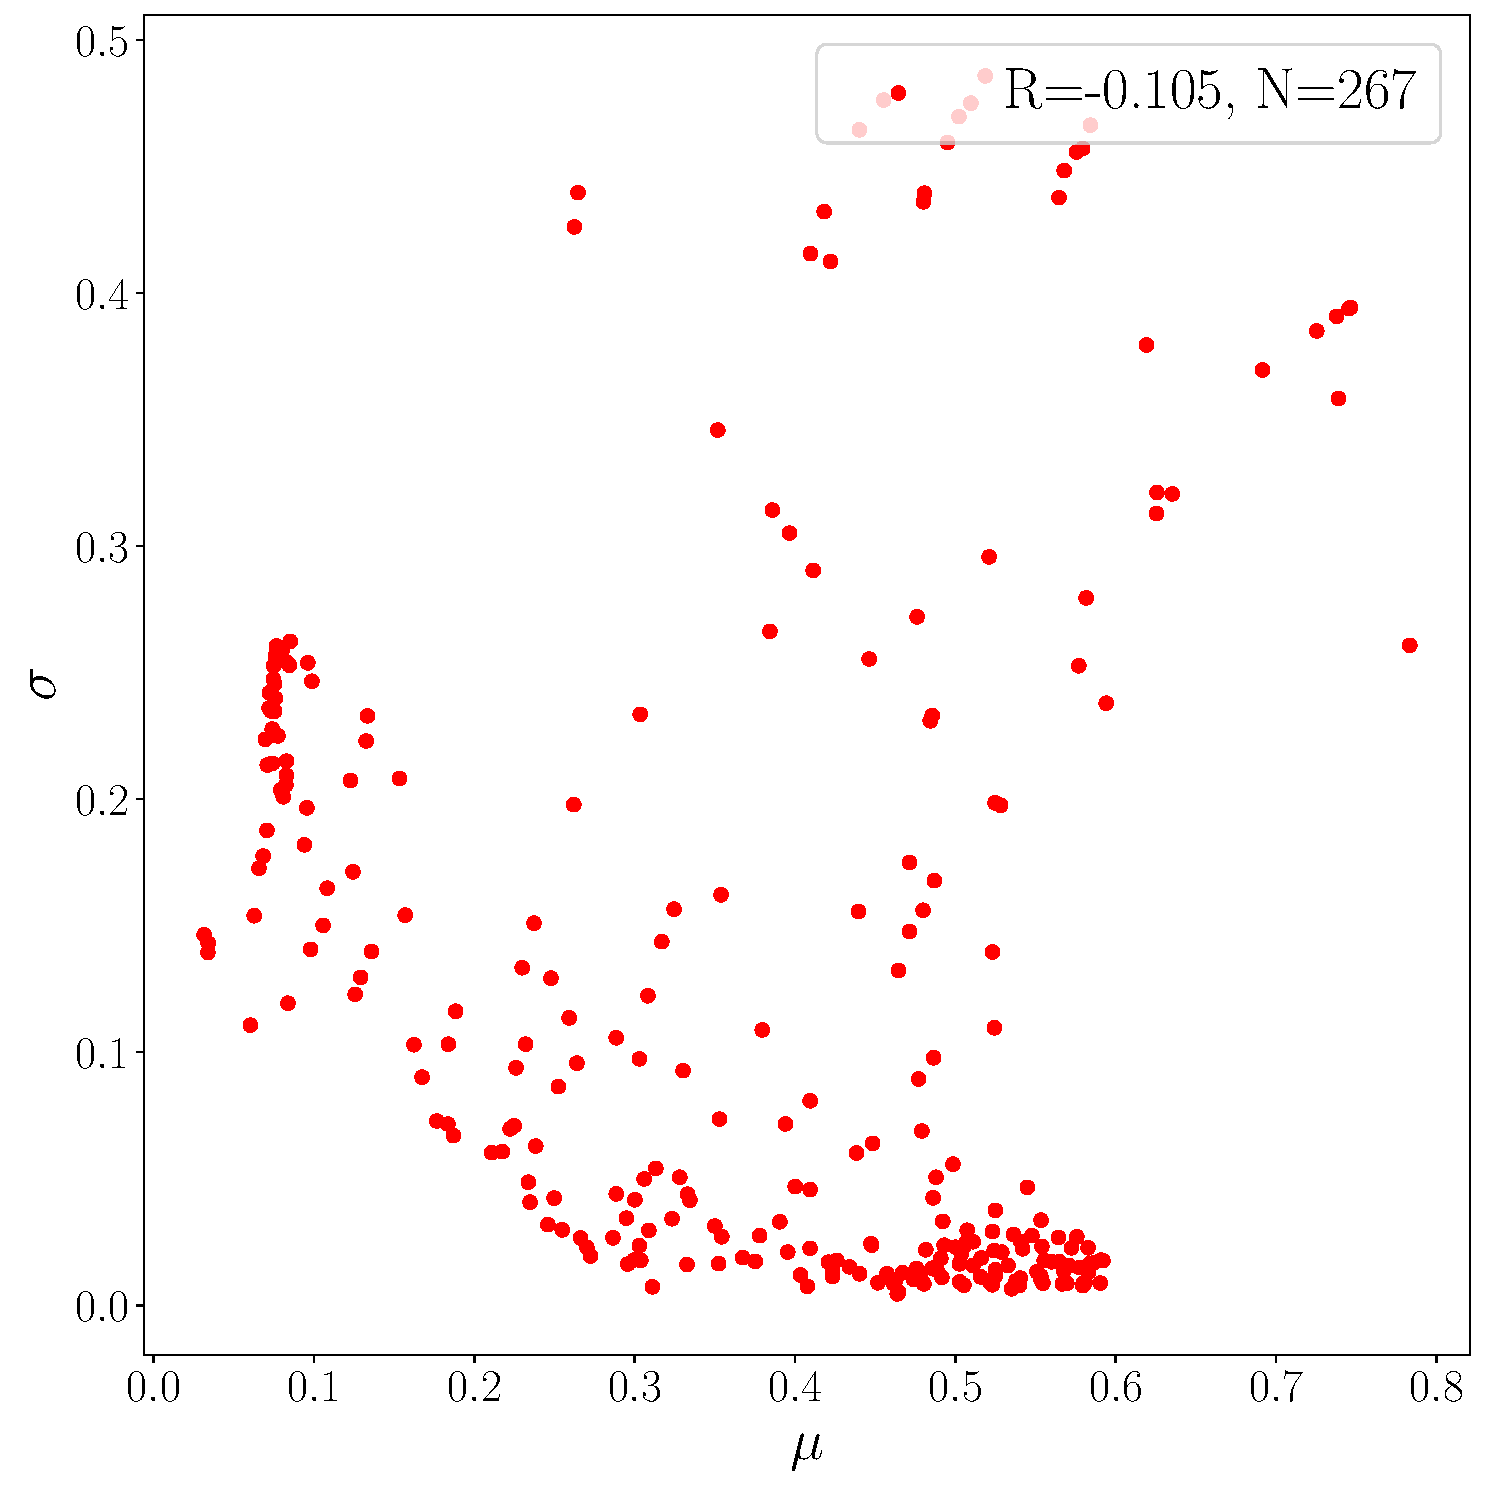
\includegraphics[width=\textwidth]{im/mu_v_sigma_}
\caption{Correlation between $\mu$ and $\sigma$.}
\end{figure}
\end{column}
\end{columns}
\end{frame}

\section{Next Steps}

\begin{frame}
\frametitle{Next Steps}
\begin{itemize}
\item Fix WILL by replacing $\Big|[k]_m - \Psi([k]_n) \Big|^q$ with $\left( 1 + \Big|[k]_m - \Psi([k]_n) \Big| \right)^q$ 
\item Try to formalise and further investigate the relationship between $\hat{Q}_\Psi$ and the extracted phase (phase extraction problem)
\item Look into adding more ILs compared to CLs 
\item Look into barren plateau mitigation techniques 
\item Explore QCNN parameter space further (number of layers,...)
\item ...? 
\end{itemize}
\end{frame}



\end{document}